%% SpatialNet -- IMWUT submission (revised draft).
%% Build: pdflatex main && bibtex main && pdflatex main && pdflatex main   (see README.md)
%% Red text marks what is still to be filled in: the real-frame check on the glasses (Section 7.8),
%% the repeated device measurements and the detector training recipe (see README.md).
\documentclass[acmsmall,screen,review,anonymous]{acmart}
\acmJournal{IMWUT}

\usepackage{multirow}
\usepackage{rotating}

%% ---- Draft markers (delete once the real-frame check and the detector recipe are filled in) ----
\newcommand{\tbd}[1]{\textcolor{red}{[#1]}}                 % text to write or confirm
\newcommand{\xx}{\textcolor{red}{xx.x}}                      % numeric result to fill in
\newcommand{\phfig}[3]{\fcolorbox{red}{white}{\parbox[c][#2][c]{\dimexpr#1-2\fboxsep-2\fboxrule\relax}{\centering\color{red}\footnotesize #3}}}

\newlength{\archh}   % height of the sideways architecture figure (set before the float)

%% ---- Notation ----
\newcommand{\vect}[1]{\mathbf{#1}}
\newcommand{\bH}{\vect{b}_h}
\newcommand{\bT}{\vect{b}_t}
\newcommand{\cH}{\vect{c}_h}
\newcommand{\cT}{\vect{c}_t}
\newcommand{\vH}{\vect{v}_h}
\newcommand{\vP}{\vect{v}_p}
\newcommand{\tip}{\vect{p}}
\newcommand{\dir}{\vect{u}}
\newcommand{\cell}{\vect{g}}

\begin{document}

\title[SpatialNet]{SpatialNet: Lightweight Pointing-Based Visual Grounding on Smart Glasses}

\author{Anonymous Author(s)}
\affiliation{%
  \institution{Anonymous Institution}
  \country{Anonymous Country}}

\begin{abstract}
Pointing is the most direct way to ask smart glasses about something in view (``what is \emph{that}?''), but resolving which object is meant currently relies on models with hundreds of millions to billions of parameters that run off the device. We ask how much of this spatial step a model small enough for the glasses can do. SpatialNet is an image-only convolutional network (0.72M parameters, 0.23 GFLOPs, 1.6\,MB in FP16) that predicts the wearer's hand, fingertip, image-plane pointing direction and the box of the pointed-at object in one forward pass. Its heads form an instance-anchored chain, and it is trained with pasted, unlabelled hands so that it keeps the wearer's hand as the reference. On the EgoPoint test split, it localises the wearer's hand with a P@0.5 of 92.6\% and the target with 58.9\%, falling to 25.4\% when the target lies far from the fingertip in the image; published models trained on EgoPoint report 63.6--93.9\% under their own protocols. Compact detectors that we trained at the same compute draw tighter boxes (59.9--67.6\%), but SpatialNet places its target centre on the labelled object more often (84.8\% against 81.6--82.2\% for four detector trainings under our recipe), and an off-the-shelf recogniser names the target from its crops as often as from the detectors' crops. Controlled experiments show what matters at this scale: input resolution is the largest lever (65.1\% at 320\,px with the same parameters); the anchored heads make the hand box and direction more precise than a plain model of the same size; training with pasted distractor hands keeps accuracy stable under synthetic hand interference, for SpatialNet and equally for a detector trained the same way; and an explicit ray prior learns mainly fingertip proximity, which neither constraining it to point forward nor up-weighting large-gap targets corrects. At least 41\% of the EgoPoint test images are COCO photographs, although COCO pretraining gains nothing extra on them. On a pre-production smart-glasses unit, the model runs in 60--80\,ms per frame.
%% Real-frame check (Section 7.8): add one clause here with the accuracy on frames from the glasses' camera.
\end{abstract}

\ccsdesc[500]{Human-centered computing~Ubiquitous and mobile computing systems and tools}
\ccsdesc[500]{Human-centered computing~Gestural input}
\ccsdesc[300]{Computing methodologies~Object detection}

\keywords{smart glasses, pointing gesture, deictic reference, egocentric vision, on-device inference, efficient neural networks}

\begin{teaserfigure}
  \centering
  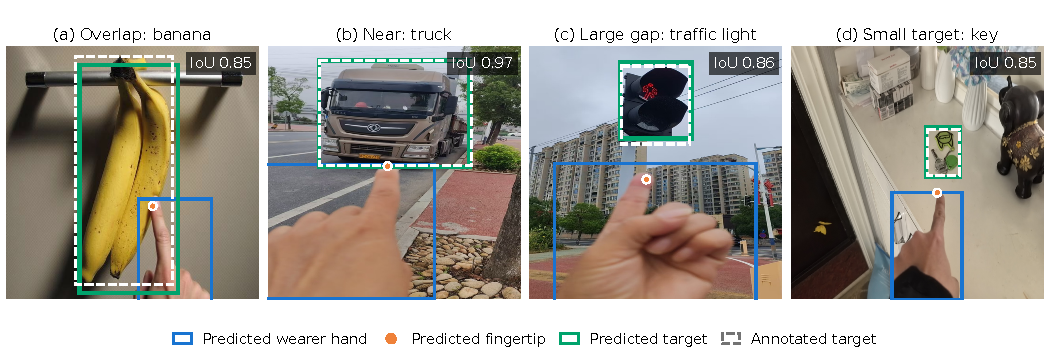
\includegraphics[width=\textwidth]{figures/teaser_successes}
  \caption{SpatialNet's predictions from a single frame: the wearer's hand (blue), the fingertip (orange) and the pointed-at object (green); white dashed: labelled object. The examples cover a target that overlaps the fingertip (a), a near target (b), a large-gap target (c) and a small large-gap target (d). Boxes, points and IoUs are the saved predictions of the 160\,px model on EgoPoint test images. These are deliberately selected successes, not average accuracy; complex failures are shown in Figure~\ref{fig:failures}.}
  \Description{Four egocentric photos with predicted boxes that match the labelled boxes: a banana touched by the finger (IoU 0.85), a truck near the fingertip (IoU 0.97), a traffic light far from the fingertip (IoU 0.86), and a small key on a wall (IoU 0.85).}
  \label{fig:teaser}
\end{teaserfigure}

\maketitle

\section{Introduction}\label{sec:intro}

Camera-equipped smart glasses are a fast-growing device category~\cite{idc2026xr,counterpoint2026aiglasses}, and an assistant on them is most useful when the wearer can refer to things in view. Pointing is the most direct way to do so: ``what is \emph{that}?'', ``remind me to buy \emph{this}''. Systems have combined speech with pointing since Bolt's \emph{Put-that-there}~\cite{bolt1980put}, and recent wearable assistants use pointing and gaze to resolve such pronouns~\cite{lee2024gazepointar}. Before any of this works on glasses, the device must answer a spatial question from its own camera: \emph{which object is the wearer pointing at?}

Three things make this hard on glasses. First, the camera sees the wearer's hand from behind and often only in part, and the target may overlap the fingertip in the image or lie far beyond it. Second, other people's hands can be in view and must not be mistaken for the wearer's. Third, the budget is small: commercial smart glasses carry batteries of a few hundred milliampere-hours that the camera, audio and radio share~\cite{yuan2026aiglasses}, while sending frames to a cloud model adds network latency and moves imagery of bystanders off the device.

Pointing-target grounding in egocentric images is an active research area, for which EgoPoint-Ground provides a large benchmark~\cite{egopoint}. The most accurate methods are large: multimodal LLMs that reason step by step from the hand to a ray and then to the target~\cite{egopoint,li2026pointvgr}, and a 226M-parameter transformer that models the pointing ray explicitly~\cite{li2026vistaref}. Some benchmark tasks even give the model the ground-truth hand box~\cite{egopoint}. These systems reach high accuracy on a GPU, but none is designed for glasses-class hardware, and to our knowledge none evaluates other people's hands in view. Egocentric fingertip systems, including one that runs on a phone, stop at the fingertip~\cite{huang2016pointing,jain2019gestarlite}, and tiny detectors that run on smart glasses find generic objects~\cite{moosmann2024tinyissimoyolo} but do not decide which one a gesture refers to.

We therefore ask how much of this spatial step a model small enough for the glasses can do. SpatialNet takes one RGB frame and nothing else: no text prompt, no hand box, no depth, and no external hand detector or pose estimator. In one forward pass of a compact convolutional network with no self-attention and no token-by-token decoding (0.72M parameters, 0.23 GFLOPs, 1.6\,MB in FP16), it predicts the wearer's hand, the fingertip, the pointing direction and the box of the pointed-at object, together with a hand-presence gate. Its design also has pointing and target gates, but EgoPoint provides no negative examples to train or test them. The model is at least 300 times smaller than VistaRef and about 10{,}000 times smaller than the 7B multimodal LLMs.

One design choice targets precision at this size: \emph{instance-anchored heads}. The heads form a chain in which each one reads a shared feature map at the location the previous one predicted, so that the fingertip, direction and target belong to the same hand. We also give the target head the geometry of the predicted ray, through a zero-initialised branch, and then test whether a model this small uses it rather than assuming so. Training pastes unlabelled hands of other people into the frames and penalises responses to them, so that the model learns to prefer the wearer's hand without labelled bystander hands.

We train and test on EgoPoint and report every target metric by the gap between the fingertip and the target in the image, because in about 70\% of images the fingertip lies inside the target box. We compare SpatialNet with published large models, with simple fingertip-based references, and with compact detectors (YOLO26n and NanoDet-Plus-m) that we trained on the same split at the same compute and scored with the same code. Because at least 41\% of the EgoPoint test images are COCO photographs, we separate detectors pretrained on COCO from those that, like SpatialNet, never saw COCO data, and test whether the overlap matters. We ablate each component, test behaviour when other people's hands are pasted into the frames, and measure latency, memory, battery drain and accuracy on the camera frames of a pre-production pair of smart glasses. We do not claim a more accurate localiser than large models, or tighter boxes than a compact detector. We show what a sub-million-parameter, image-only model can do on smart-glasses hardware, where it fails, and which design choices matter at that scale.

\paragraph{Contributions.}
\begin{enumerate}
\item \emph{A deployable, image-only pointing-target localiser for smart glasses.} A 0.72M-parameter CNN returns the wearer's hand, fingertip, direction and target box in one pass, and runs in 60--80\,ms per frame on a pre-production glasses unit, where we also check its accuracy on the unit's own camera frames (Sections~\ref{sec:method}, \ref{sec:device}, \ref{sec:ondevice} and~\ref{sec:realframes}).
%% If the real-frame check (Section 7.8) cannot be done in time, delete the clause ", where we also check ...", and Section 7.8.
\item \emph{A controlled characterisation of accuracy against cost at wearable scale.} Beyond published large models, we compare with compact detectors trained under our protocol, including a pretraining control, and report an end-to-end score, a resolution study, results by fingertip--target gap, retraining variation and a duplicate audit. At the same compute and with the same ImageNet pretraining, a detector draws tighter boxes (63.2\% against 58.9\% P@0.5), but SpatialNet places its target centre on the labelled object more often (84.8\% against 81.6--82.2\% for four detector trainings, all paired intervals excluding zero), and in a downstream test an off-the-shelf recogniser names the target from SpatialNet's crops as often as from the detectors', except when the target lies far from the fingertip. We also show that at least 41\% of the EgoPoint test images are COCO train2014 photographs, which any benchmark on this dataset should report, although COCO pretraining gains nothing extra on them (Sections~\ref{sec:data} and \ref{sec:main}--\ref{sec:heads-results}).
\item \emph{Mechanism-level findings for small pointing models.} Input resolution is the largest lever, at no parameter cost. Instance anchoring makes the hand box and the direction more precise than a plain model of the same size, without changing coarse accuracy. Distractor pasting keeps accuracy under synthetic interference at no cost on clean images, and the recipe transfers unchanged to a generic detector. An explicit ray prior learns mainly fingertip proximity when most targets overlap the fingertip; neither constraining it to point forward, nor up-weighting large-gap targets, nor widening the size sample fixes large-gap or box-extent errors (Sections~\ref{sec:detectors} and \ref{sec:resolution}--\ref{sec:own}).
\end{enumerate}

\section{Related Work}\label{sec:related}

\paragraph{Pointing as input.} Deictic gestures have been part of multimodal interfaces since \emph{Put-that-there}~\cite{bolt1980put}. Ray-casting is a standard way to select objects in virtual and augmented reality~\cite{argelaguet2013survey}, and studies of mid-air pointing show that both the hand and the eye matter: ray-casting models have systematic offsets~\cite{mayer2015modeling}, accounting for the dominant eye makes them markedly more accurate~\cite{plaumann2018towards}, and visual feedback such as a cursor improves accuracy further~\cite{mayer2018effect}. On smart glasses, the small form factor limits the input options~\cite{lee2018interaction}. GazePointAR combines gaze, pointing and conversation history to resolve spoken pronouns in AR~\cite{lee2024gazepointar}, and EgoPointVQA answers questions about pointed-at objects in egocentric video by feeding 3D hand keypoints, estimated by an off-the-shelf model, to a multimodal LLM~\cite{choi2026hint}. These systems show the value of pointing on wearables; SpatialNet supplies the localisation step they need, at a cost that fits on the glasses.

\paragraph{Hands, fingertips and directions.} EgoFinger detects the hand and fingertip in egocentric video for air-writing~\cite{huang2016pointing}, and GestARLite runs a hand detector, a fingertip regressor and a gesture classifier on a smartphone~\cite{jain2019gestarlite}. On-device trackers estimate full hand keypoints in real time on phones~\cite{zhang2020mediapipe} and on headsets~\cite{han2020megatrack}, and DeePoint estimates the 3D pointing direction from third-person video of the whole body~\cite{nakamura2023deepoint}. None of these localises the object being pointed at. Egocentric hand datasets have long distinguished the wearer's hands from other people's: EgoHands labels \emph{my} and \emph{your} left and right hands~\cite{bambach2015lending}, and large-scale detectors model hand side and contact state~\cite{shan2020understanding}. Pointing datasets, EgoPoint included, contain only the wearer's hand, so we synthesise other people's hands with copy-paste augmentation~\cite{dwibedi2017cut,ghiasi2021simple}; unlike in standard copy-paste, the pasted instances are deliberately left unlabelled and penalised.

\paragraph{Pointing-target grounding.} YouRefIt grounds targets from language and gesture together in third-person views~\cite{chen2021yourefit}. For egocentric images, EgoPoint-Ground introduced 15K images (real captures from smart glasses, plus synthetically composed and generated images) and several tasks~\cite{egopoint}. In its pointing-only task, models receive the image and the ground-truth hand box and are evaluated without task-specific training, and its SV-CoT baseline reasons with a multimodal LLM from the pointing direction to a ray and then to the target. PointVG-R builds a similar hand--direction--ray--target chain of thought into Qwen2.5-VL-7B with reinforcement learning, and names latency as a limitation for wearables~\cite{li2026pointvgr}. VistaRef adds hand-keypoint and geometric-ray modules and an orientation-consistency loss to a BEiT-3 grounding model (226M parameters with the Base backbone) and, with the Large backbone, reports a P@0.5 of 93.9\% on the 3,072 EgoPoint test images~\cite{li2026vistaref}. EgoPoint-Bench shows that general multimodal LLMs still struggle with egocentric pointing~\cite{li2026egopointbench}. Explicit ray reasoning is thus not new, and neither is avoiding a hand-box input: VistaRef uses a fixed prompt and finds the hand itself. What differs here is the operating point, an image-only, single-pass CNN 300 to 10{,}000 times smaller that runs on smart-glasses hardware, and a test of whether explicit ray geometry helps a model this small. Table~\ref{tab:related} summarises the differences.

\paragraph{Efficient models and compact detectors.} Our trunk follows efficient detection design~\cite{ma2018shufflenet,tan2020efficientdet}, and our heads predict keypoint heatmaps in the manner of CenterNet~\cite{zhou2019objects}, with a differentiable soft-argmax~\cite{sun2018integral}. Tiny networks now run on microcontrollers~\cite{lin2020mcunet} and, for generic object detection, on smart glasses~\cite{moosmann2024tinyissimoyolo}. A compact detector such as YOLO26n~\cite{ultralytics2026yolo26} or NanoDet-Plus~\cite{rangilyu2021nanodet}, trained on pointing data to box the pointed-at object, needs no pointing-specific structure at all; we therefore use such detectors as baselines at matched compute (Section~\ref{sec:detectors}). Open-vocabulary detectors and multimodal LLMs can ground text queries~\cite{liu2024grounding,peng2023kosmos,you2024ferret,bai2025qwen25vl}, but pointing is not text, and their size rules them out for continuous use on glasses.

\begin{table}[t]
  \caption{Methods that localise pointing or its target. \emph{Hand box}: the ground-truth hand box is an input. Parameter counts as reported; ``$>$1B'': built on a multimodal LLM.}
  \label{tab:related}
  \footnotesize
  \setlength{\tabcolsep}{3pt}
  \begin{tabular}{lllllll}
    \toprule
    Method & View & Test-time input & Output & Params & On device & Other hands \\
    \midrule
    EgoFinger~\cite{huang2016pointing} & ego & image & fingertip & -- & -- & -- \\
    GestARLite~\cite{jain2019gestarlite} & ego & frames & fingertip, gesture & 16.3\,MB & phone & -- \\
    DeePoint~\cite{nakamura2023deepoint} & 3rd & video & pointing, 3D direction & -- & -- & -- \\
    YouRefIt~\cite{chen2021yourefit} & 3rd & image + language & target box & -- & -- & -- \\
    SV-CoT (POG)~\cite{egopoint} & ego & image + hand box & target box & $>$1B & -- & -- \\
    PointVG-R~\cite{li2026pointvgr} & ego & image + instruction & target box & 7B & -- & -- \\
    VistaRef~\cite{li2026vistaref} & ego & image + fixed prompt & target box, keypoints & $\geq$226M & -- & -- \\
    \textbf{SpatialNet} & ego & image & hand, tip, ray, target & 0.72M & glasses & trained \\
    \bottomrule
  \end{tabular}
\end{table}

\section{Problem Definition}\label{sec:problem}

\paragraph{Outputs.} Given one RGB frame from a head-worn camera, SpatialNet predicts:
\begin{enumerate}
\item three presence flags $(H,P,T)$: the wearer's hand is visible, the hand is pointing, and something is pointed at;
\item the box $\bH$ of the wearer's hand;
\item the fingertip $\tip$;
\item the pointing direction $\dir$ in the image plane;
\item the box $\bT$ of the pointed-at object, which we call the \emph{target}.
\end{enumerate}
Boxes are $(c_x,c_y,w,h)$ and points $(x,y)$, both normalised to $[0,1]$. The flags combine into four scenes that an interface can act on: 000 \emph{no hand}, 100 \emph{hand, not pointing}, 110 \emph{pointing, no target} and 111 \emph{pointing at a target}. EgoPoint contains only scenes 000 and 111 (Section~\ref{sec:data}). We therefore train and evaluate SpatialNet as a two-scene model: the pointing and target gates are part of the interface design, but they receive no negative examples and are not evaluated.

\paragraph{Fingertip--target gap.} We describe each target by its gap to the fingertip in the image: \emph{overlap} when the fingertip lies inside the target box, \emph{near} when the shortest fingertip--box distance is at most 0.08 of the image side, and \emph{large gap} otherwise. These are image-plane relations: an overlap does not imply that the finger touches the object, and a large gap does not imply that the object is far from the wearer.

\paragraph{What separates this from generic detection.} \emph{Ownership}: when several hands are visible, $\bH$, $\tip$ and $\bT$ must refer to the wearer's hand, and a frame showing only other people's hands is \emph{no hand}. \emph{Budget}: the model must run on the glasses' own processor, without a second network or a server call, within the 100--200\,ms commonly targeted for interactive response~\cite{miller1968response,card1991information}.

\paragraph{Scope.} We do not recognise \emph{what} the target is. $\bT$ is the region that a later step would take as input: an object recogniser, a visual question-answering model or an application. Localising the region first means that this step can run on a small crop instead of the full frame, and only when the wearer's hand is detected. The cost of that later step is outside the scope of this paper, but we test how well an off-the-shelf recogniser names the target from each model's crop (Section~\ref{sec:detectors}).

\section{SpatialNet}\label{sec:method}

Figure~\ref{fig:arch} shows the complete network. A shared trunk turns the frame into one feature map. Four heads then run in a fixed order (wearer's hand, fingertip, pointing direction, pointed target), and each head reads the shared map \emph{at the location that the previous head predicted}. We call these heads \emph{instance-anchored}: the fingertip is searched for around the hand that was found, the direction is computed from features of that hand and fingertip, and the target is searched for along the resulting ray. Three small gates decide which outputs are valid. Everything is a single forward pass; there is no external hand detector, no language input, and no hand box at test time.

\begin{figure}[t]
  \centering
  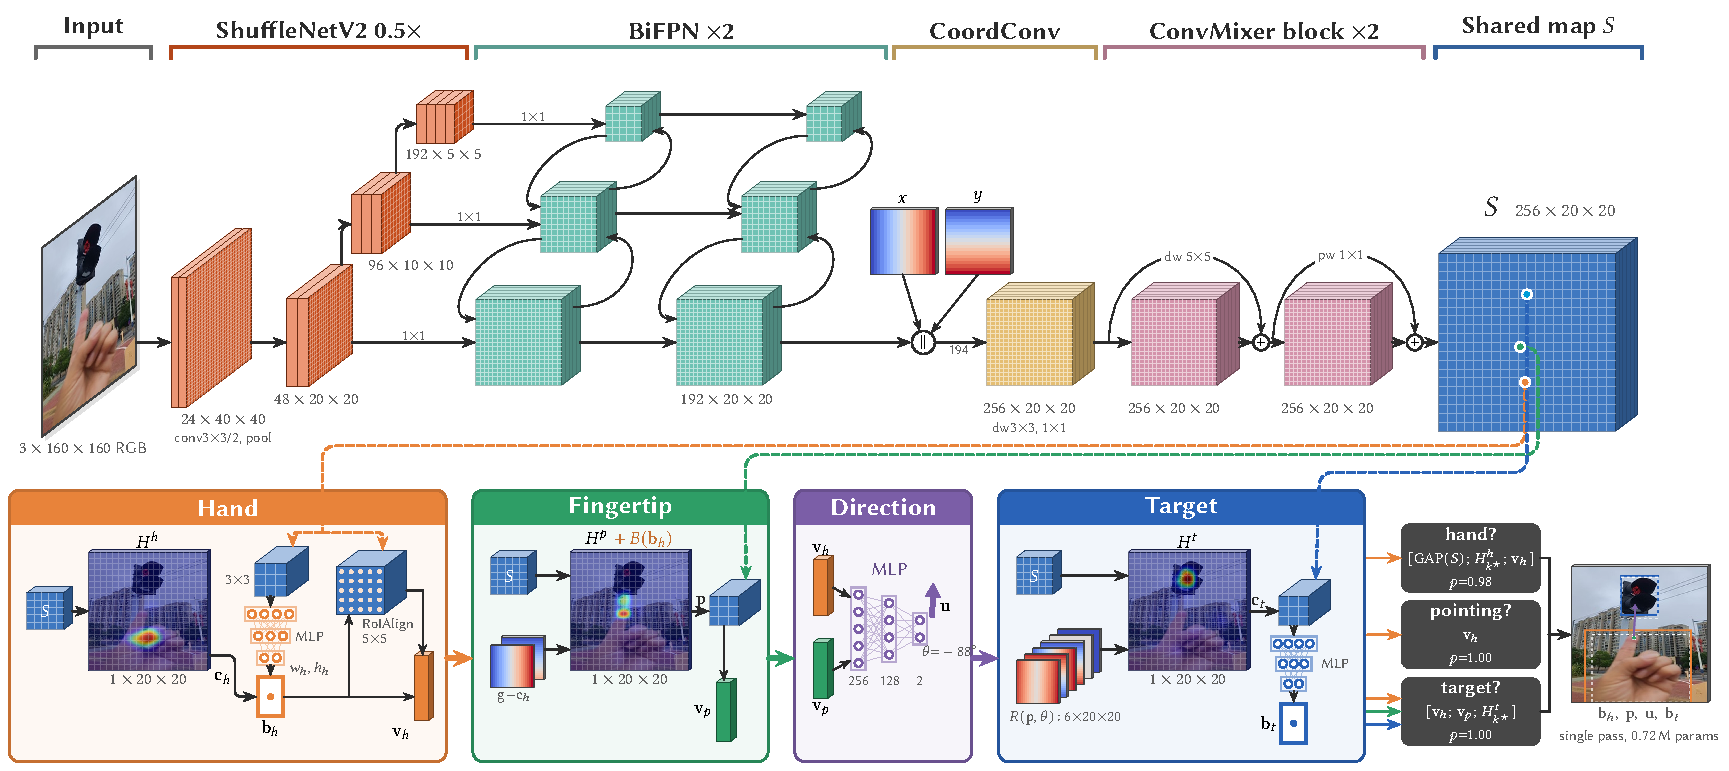
\includegraphics[width=\textwidth]{figures/architecture}
  \caption{SpatialNet. The trunk (top) turns one $160\times160$ frame into the shared map $S$ ($256\times20\times20$): ShuffleNetV2 stages at strides 8, 16 and 32, two BiFPN layers, CoordConv with reduction to 256 channels, and two ConvMixer blocks. Four heads (middle) run in order. Dashed lines mark where a head samples $S$ at the location the previous head predicted: the hand centre $\cH$, the fingertip $\tip$ and the target centre $\cT$. The direction head reads only the descriptors $\vH,\vP$. Right: the presence gates and the decoded output. Heatmaps, offset and ray-coordinate maps, gate probabilities and the output are real outputs of the trained model on one test image; each heatmap is overlaid on the input frame and scaled to its maximum.}
  \Description{Block diagram drawn as three-dimensional tensor slabs. The input frame passes through a ShuffleNetV2 backbone whose three scales feed two BiFPN layers by 1x1 projections; the 20x20 output gets two coordinate channels, is reduced to 256 channels and passes two ConvMixer blocks to give the shared map S. Four coloured panels show the heads in sequence: wearer hand (heatmap, 3x3 sample and MLP for the box size, RoIAlign descriptor), fingertip (heatmap from S and offset channels to the hand centre plus a hand-box prior, 3x3 sample giving the fingertip descriptor), pointing direction (an MLP on the hand and fingertip descriptors giving a unit vector), and pointed target (six ray-coordinate maps and S giving the target heatmap, 3x3 sample and MLP giving the box). Dashed lines from S show where each head samples it. On the right, three presence gates list their inputs and probabilities, and the output frame shows the predicted hand box, fingertip, direction and target box.}
  \label{fig:arch}
\end{figure}

\subsection{Shared Trunk}\label{sec:trunk}
The frame is resized to $160\times160$. A ShuffleNetV2~0.5$\times$ backbone~\cite{ma2018shufflenet} (stages 2--4 only; ImageNet-pretrained~\cite{deng2009imagenet}) gives feature maps at strides 8, 16 and 32. Two BiFPN layers~\cite{tan2020efficientdet} merge them into one $192\times20\times20$ map at stride 8. Each fused map is smoothed by a depthwise $3\times3$ convolution, SiLU, and parameter-free SimAM attention~\cite{yang2021simam}. We then append two coordinate channels (CoordConv~\cite{liu2018coordconv}) and reduce to $D{=}256$ channels with a depthwise-separable convolution. Two ConvMixer-style residual blocks~\cite{trockman2023patches} follow, each made of a depthwise $5\times5$ and a pointwise convolution with residual connections; their batch-norm scales start at zero, so each block is the identity at initialisation. The output is the shared map $S\in\mathbb{R}^{256\times20\times20}$, which all heads read. A $20\times20$ grid gives 8-pixel cells at the model input; the heads recover points with sub-cell precision (Section~\ref{sec:softargmax}), so a finer grid would mostly add compute. Sharing one map keeps the heads cheap: the largest head has 104K parameters (Table~\ref{tab:params}).

\subsection{Locating One Instance: Peak-Windowed Soft-Argmax}\label{sec:softargmax}
Each head predicts a $20\times20$ logit map $H$ and turns it into a point. A global soft-argmax~\cite{sun2018integral} returns the probability-weighted mean over all cells; when two hands are visible, that mean falls \emph{between} them. We therefore restrict the softmax to a $(2r{+}1)\times(2r{+}1)$ window $\mathcal{W}$ around the arg-max cell $k^\star$:
\begin{equation}
\pi_k=\frac{\mathbb{1}[k\in\mathcal{W}]\,\exp(\tau H_k)}{\sum_{j\in\mathcal{W}}\exp(\tau H_j)},\qquad
\hat{\vect{c}}=\sum_k \pi_k\,\cell_k ,
\label{eq:softargmax}
\end{equation}
where $\cell_k\in[0,1]^2$ is the normalised position of cell $k$ and $\tau$ is a temperature. The estimate follows a single peak, is differentiable within the window, and is not limited to cell centres. We use $(\tau,r)=(8,2)$ for the hand and the target and $(10,1)$ for the fingertip. The peak logit $H_{k^\star}$ is also passed to the gates as a confidence cue.

\subsection{Instance-Anchored Heads}\label{sec:heads}

\paragraph{Wearer's hand.} A depthwise $3\times3$ and pointwise head gives hand-centre logits $H^h$, and Eq.~\eqref{eq:softargmax} gives the centre $\cH$. For the box size $(w_h,h_h)$, we sample a $3\times3$ neighbourhood of $S$ around $\cH$ bilinearly (one-cell spacing). A depthwise $3\times3$ convolution and a pointwise projection collapse it to 128 dimensions, and a two-layer MLP with a sigmoid maps it to the size, giving $\bH=(\cH,w_h,h_h)$. To describe \emph{this} hand instance, we sample a $5\times5$ RoIAlign-style lattice~\cite{he2017mask} over $\bH$ enlarged by 1.15, collapse it to 128 dimensions, and fuse it with the box coordinates into the hand descriptor $\vH\in\mathbb{R}^{128}$.

\paragraph{Fingertip.} The fingertip must belong to the hand just found. Its logits add three terms:
\begin{equation}
H^p = V^p(S) + G^p\big([S;\,\alpha_p(\cell-\cH)]\big) + B(\bH).
\label{eq:tip}
\end{equation}
$V^p$ is a visual head of the same form as the hand head. $\alpha_p(\cell-\cH)$ are two channels holding each cell's offset to the hand centre, with a learnable scale $\alpha_p$, and $G^p$ is a small branch (a $1\times1$ convolution to 48 channels, then a $3\times3$ convolution to one channel, with its last layer initialised at zero) that learns where fingertips lie relative to the hand centre. $B$ is a fixed log-prior that is zero inside the hand box dilated by $\delta{=}1.3$ and falls linearly outside it:
\begin{equation}
B_k(\bH) = -\frac{\lambda}{\tau_p}\Big(\big[\tfrac{|g_{k,x}-c_{h,x}|}{\delta w_h/2}-1\big]_+ + \big[\tfrac{|g_{k,y}-c_{h,y}|}{\delta h_h/2}-1\big]_+\Big),
\end{equation}
where $[\cdot]_+=\max(\cdot,0)$. With $\lambda{=}4$, the penalty after the softmax temperature $\tau_p$ is 4 logits for every half box-width outside the dilated box, and no gradient flows from the prior into $\bH$. In the training labels, the fingertip lies inside the dilated box in 99.4\% of pointing images, so the prior rarely contradicts a label while it rules out the fingertips of other hands. Eq.~\eqref{eq:softargmax} (with $r{=}1$) gives the fingertip $\tip$, and a $3\times3$ sample around it gives the fingertip descriptor $\vP\in\mathbb{R}^{128}$.

\paragraph{Pointing direction.} An MLP ($256\to128\to2$, $\tanh$) maps $[\vH;\vP]$ to a vector, which we L2-normalise into the unit direction $\dir=(\cos\theta,\sin\theta)$ in image coordinates. The direction is supervised with the image-plane direction from the labelled fingertip to the labelled target centre (Section~\ref{sec:losses}), so $\dir$ is the direction \emph{to the target} as it appears in the image, not the 3D orientation of the finger.

\paragraph{Pointed target.} The target head is given the geometry of the predicted ray explicitly. From $\tip$ and $\dir$, every cell $k$ receives six \emph{ray coordinates} (inset in Figure~\ref{fig:arch}):
\begin{equation}
\Delta_k=\alpha_t(\cell_k-\tip),\qquad
t_k=\Delta_k\cdot\dir,\qquad
s_k=\big|\Delta_{k,x}\sin\theta-\Delta_{k,y}\cos\theta\big|,\qquad
\cos\theta,\qquad \sin\theta .
\label{eq:raycoords}
\end{equation}
These are the scaled offset from the fingertip (two channels), the signed distance along the ray (negative behind the fingertip), the distance from the line of the ray, and the direction itself. The target logits are
\begin{equation}
H^t = V^t(S) + G^t\big([S;\,R(\tip,\theta)]\big),
\label{eq:target}
\end{equation}
where $R$ stacks the six maps, and $G^t$ (13K parameters) has the form of $G^p$ and also starts at zero. The soft-argmax applies a softmax to $\tau H^t$, so $\pi_k\propto\exp(\tau V^t_k)\exp(\tau G^t_k)$: the geometry term acts as a learned \emph{multiplicative prior} on the visual evidence. Because $G^t$ starts at zero, training begins with a purely visual head, and the network uses the ray only as far as it lowers the loss. We let the network learn the shape of this prior, instead of fixing a cone, because the right shape depends on the gap: when the fingertip overlaps the target (about 70\% of EgoPoint targets, Section~\ref{sec:data}), the target centre can lie in any direction from the fingertip, while for large-gap targets a narrow band along the ray is informative. Whether the network exploits this freedom is an empirical question; Section~\ref{sec:ablations} shows that on EgoPoint it learns mainly a fingertip-proximity prior. The target centre $\cT$ follows from Eq.~\eqref{eq:softargmax}, and its size comes from a $3\times3$ sample, as for the hand, giving $\bT=(\cT,w_t,h_t)$.

\begin{table}[t]
  \caption{Parameters per module. FLOPs are counted by PyTorch's \texttt{FlopCounterMode} (one multiply--accumulate = 2 FLOPs; bilinear sampling not counted) for one $160\times160$ frame. Sizes are serialised state dictionaries.}
  \label{tab:params}
  \small
  \begin{tabular}{lrl}
    \toprule
    Module & Parameters & Role \\
    \midrule
    ShuffleNetV2 0.5$\times$, stages 2--4 & 143,136 & backbone, ImageNet-pretrained \\
    BiFPN $\times2$ & 81,426 & multi-scale fusion to stride 8 \\
    CoordConv + reduce & 52,310 & $194\to256$ channels \\
    ConvMixer $\times2$ & 145,920 & context mixing ($5\times5$ depthwise) \\
    \midrule
    Hand head & 104,259 & heatmap, size, descriptor $\vH$ \\
    Fingertip head & 51,826 & incl.\ 12,913 in the hand-offset branch $G^p$ \\
    Direction MLP & 33,154 & $[\vH;\vP]\to\dir$ \\
    Target head & 60,404 & incl.\ 13,105 in the ray branch $G^t$ \\
    Gates (hand / pointing / target) & 24,769 / 8,321 / 16,577 & presence logits \\
    Learnable scales $\alpha_p,\alpha_t$ & 2 & \\
    \midrule
    \textbf{Total} & \textbf{722,104} & 0.231 GFLOPs; 3.0\,MB FP32; 1.6\,MB FP16 \\
    \bottomrule
  \end{tabular}
\end{table}

\subsection{Presence Gates and Scene Decoding}\label{sec:gates}
Three MLP gates output logits for whether the wearer's hand is present (from $[\mathrm{GAP}(S);\,H^h_{k^\star};\,\vH]$), whether it is pointing (from $\vH$ alone) and whether something is pointed at (from $[\vH;\vP;H^t_{k^\star}]$). At inference they form a cascade with threshold 0.5: if the hand gate is off, the frame is \emph{no hand}; otherwise the pointing gate and then the target gate decide between \emph{hand, not pointing}, \emph{pointing, no target} and \emph{pointing at a target}. The pointing and target gates read instance descriptors rather than the whole image, so that another person's pointing hand elsewhere in the frame is not meant to switch them on by itself. The hand gate also sees the global pool, so that a frame containing only other people's hands can be classed as having \emph{no wearer's hand}. EgoPoint contains only the first and last of the four scenes (Section~\ref{sec:data}), so we evaluate the hand gate and make no claims about the pointing and target gates.

\subsection{Training Objective}\label{sec:losses}
The loss is a weighted sum of 13 terms (weights in Appendix~\ref{app:weights}), each computed only on images whose label contains the parts it needs. \emph{Localisation} uses the CIoU loss for the hand box~\cite{zheng2020distance}; the Wing loss~\cite{feng2018wing} for the fingertip, on normalised coordinates with $w{=}0.5$ and $\epsilon{=}0.1$; $1-\cos(\dir,\dir^\star)$ for the direction, where $\dir^\star$ is the unit vector from the labelled fingertip to the labelled target centre; and the SIoU loss~\cite{gevorgyan2022siou} plus $1-\mathrm{IoU}$ for the target box. \emph{Heatmaps} use the penalty-reduced focal loss of CornerNet and CenterNet~\cite{law2018cornernet,zhou2019objects} ($\alpha{=}2$, $\beta{=}4$) on Gaussian targets at the hand centre, fingertip and target centre ($\sigma$ = 1.5, 0.8 and 1.2 cells), which gives each heatmap a direct signal in addition to the gradient through the soft-argmax. \emph{Gates} use focal binary cross-entropy~\cite{lin2017focal} ($\gamma{=}2$), each on its own population (the hand gate on all images, the pointing gate on hand images, the target gate on pointing images), with positives weighted $2\times$ ($3\times$ for the hand gate), because a missed pointing gesture costs the user more than a false alarm that the interface can ignore.

\emph{Geometric consistency} adds two terms that use predictions only. The ray-alignment term asks the predicted target centre to lie on the predicted ray, in front of the fingertip:
\begin{equation}
\mathcal{L}_{\mathrm{ray}} = \big\|\vect{r}-(\vect{r}\cdot\hat{\dir})\,\hat{\dir}\big\| + 0.5\,\big[-\vect{r}\cdot\hat{\dir}\big]_+,\qquad \vect{r}=\hat{\vect{c}}_t-\hat{\tip}.
\end{equation}
Because $\dir^\star$ runs from the labelled fingertip to the labelled target centre, the ground truth gives $\mathcal{L}_{\mathrm{ray}}=0$ exactly: the term does not move the optimum and only penalises predictions that disagree with each other. For a fixed angular error, it grows with the fingertip--target distance, so it weighs large-gap targets most. The hand-axis term is a hinge that keeps $\hat{\dir}$ within $60^\circ$ of the axis from the predicted hand centre to the predicted fingertip. It is only a weak plausibility prior: the labelled direction lies inside this cone in 68.6\% of training images (64.1\% for overlap targets and 83.6\% for large-gap targets), so it has the smallest weight of all 13 terms. Ablation A2 (Section~\ref{sec:ablations}) removes both consistency terms.

\subsection{Learning Whose Hand It Is}\label{sec:ownership}
No public pointing dataset labels other people's hands, and EgoPoint frames contain only the wearer's. We therefore create distractors during training (Figure~\ref{fig:ownership}). The approach follows copy-paste augmentation~\cite{dwibedi2017cut,ghiasi2021simple}, but with the opposite aim: pasted hands are \emph{not} labelled, and the model is penalised for responding to them.

\begin{figure}[t]
  \centering
  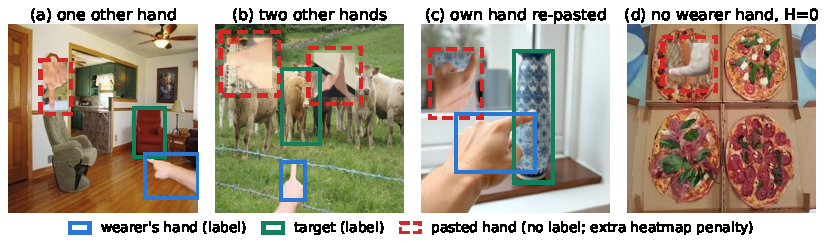
\includegraphics[width=\linewidth]{figures/ownership_examples}
  \caption{Distractor-hand pasting, produced by the training code. Pasted hands (red, dashed) come from other images (a, b) or from the same image (c), are rotated so that they rarely enter from the bottom edge, and are never labelled. A no-hand image with a pasted hand keeps the label \emph{no hand} (d).}
  \Description{Four training images. In the first two, one or two hands cut from other photos are pasted into the upper part of the image, rotated, and marked with red dashed boxes, while the wearer's pointing hand and the target keep their blue and green label boxes. In the third, a rotated copy of the wearer's own hand is pasted in the upper left. In the fourth, a pizza photo without a wearer's hand receives a pasted hand and keeps the label no hand.}
  \label{fig:ownership}
\end{figure}

With probability 0.5 for images with a hand and 0.3 for images without one, we paste one or two hand crops taken from other training images. The crops are rescaled, usually rotated (so that, unlike the wearer's arm, they rarely enter from the bottom edge), centred in the upper 65\% of the frame away from the wearer's hand and the target, and blended with a feathered mask; Appendix~\ref{app:aug} lists all settings. In 30\% of cases the pasted crop is the wearer's own hand from the same image, so that appearance alone cannot tell the two hands apart and the model has to use position, orientation and context. With probability 0.15, we also paste an unlabelled patch that contains no hand, so that a pasted rectangle is not itself a cue. Labels never change: in particular, a no-hand image with pasted hands remains \emph{no hand}, which teaches the hand gate to answer for the wearer only. In the hand-heatmap loss, the negative term near a pasted hand is multiplied by $1+4\,G_k$, where $G_k$ is a Gaussian ($\sigma{=}1.5$ cells) at that hand's centre, so that a response on another person's hand costs up to five times as much as one on background.

\emph{The prior this encodes.} The procedure assumes that, from a head-worn camera, the wearer's arm enters from the bottom of the frame, while other people's hands appear higher and in other orientations. This holds for most use of glasses but not always, for example when the wearer raises a hand above eye level or when a companion's hand is near the bottom of the view (Section~\ref{sec:discussion}).

\subsection{Scheduled Anchor Forcing}\label{sec:forcing}
Early in training, the predicted hand centre, fingertip and target centre are close to random, so the downstream heads would read features at meaningless locations. As in scheduled sampling for sequence models~\cite{bengio2015scheduled}, we sometimes replace each anchor with its ground-truth location, independently per image and per anchor, with a probability that decreases linearly from 0.5 to 0 over the first 20 epochs. From then on, training uses the model's own anchors, as at test time.

\section{Data and Evaluation Protocol}\label{sec:data}

\subsection{EgoPoint}
We train and test on the image set of EgoPoint-Ground~\cite{egopoint}, which we call EgoPoint. Its paper reports 15,338 images: 39\% (6,035) real captures with RayNeo~V3 smart glasses (12\,MP Sony IMX681 sensor), 39\% (5,976) synthetically composed and 22\% (3,327) LLM-generated; its appendix calls the last two groups ``synthetic generation'' and ``image editing''. The edited images were made from third-person photographs of COCO~\cite{lin2014coco}, selected through the RefCOCO referring-expression dataset~\cite{yu2016modeling}, into which a multimodal model added a pointing hand~\cite{egopoint}. The release we use has 15,455 images split 10,837 / 1,546 / 3,072. VistaRef~\cite{li2026vistaref} and PointVG-R~\cite{li2026pointvgr} report the same counts, so our test images are theirs, minus the exclusions below. The release does not mark which images are real captures and which are generated, so, like VistaRef and PointVG-R, we report on the whole test split. It does, however, name the source photograph of each edited image. In our test split, 842 of the 2,604 images with a target (32\%) are edited COCO train2014 photographs, and at least 400 of the 425 no-hand images are unedited COCO train2014 photographs, so at least 1,242 test images (41\%) come from COCO. This matters for baselines pretrained on COCO (Section~\ref{sec:metrics}). Each positive record shows one wearer's hand pointing at one target; negatives show no hand.

\paragraph{Conversion.} Negatives become 000, and their object boxes are ignored; positives with a hand box, an annotated fingertip and a target box become 111. In three test records, the hand label was attached to an object and the hand was labelled as an object; we detected these by the fingertip position and swapped the labels back. We dropped 232 positives: 229 without an annotated fingertip (164 train, 22 validation, 43 test), all flagged as unclear in the source annotations, and 3 without a hand box. Spot checks showed open palms, held objects, or a hand box on the hand that was not pointing. If all 43 dropped test positives were counted as failures, the target P@0.5 reported in Section~\ref{sec:results} would fall by less than one point, to about 58\%. Table~\ref{tab:data} summarises the result. Images are stored at $224\times224$; the model squashes every frame to its square $160\times160$ input, regardless of the original aspect ratio.

\begin{table}[t]
  \caption{EgoPoint after conversion. Gap categories (Section~\ref{sec:problem}): \emph{overlap}, the fingertip lies inside the target box; \emph{near}, fingertip--box distance ${\leq}\,0.08$ of the image side; \emph{large gap}, ${>}\,0.08$.}
  \label{tab:data}
  \footnotesize
  \begin{tabular}{lrrrrrr}
    \toprule
    & & & & \multicolumn{3}{c}{Pointing at target, by gap} \\
    \cmidrule(l){5-7}
    Split & Images & No hand (000) & Pointing at target (111) & Overlap & Near & Large gap \\
    \midrule
    Train & 10,669 & 1,535 & 9,134 & 6,511 & 1,995 & 628 \\
    Validation & 1,524 & 211 & 1,313 & 922 & 297 & 94 \\
    Test & 3,029 & 425 & 2,604 & 1,796 & 599 & 209 \\
    \midrule
    Total & 15,222 & 2,171 & 13,051 & 9,229 & 2,891 & 931 \\
    \bottomrule
  \end{tabular}
\end{table}

\paragraph{Consequences for evaluation.} Our test split has 3,029 images, 43 positives fewer than the official one, and published numbers on the official split are not strictly comparable with ours (Section~\ref{sec:main}). EgoPoint contains only scenes 000 and 111, so the pointing and target gates never see a negative example, and we report neither their accuracy nor four-class scene accuracy. About 70\% of targets overlap the fingertip and only 7\% have a large gap. Pooled results are dominated by overlap targets, so we report every target metric by gap as well. The median distance from the fingertip to the target centre is 0.12, 0.17 and 0.32 of the image side for overlap, near and large-gap targets (test split).

\subsection{Metrics}\label{sec:metrics}
\begin{itemize}
\item \emph{Target and hand localisation.} We use the two standard grounding metrics~\cite{egopoint,li2026vistaref,li2026pointvgr}: \emph{mIoU}, the IoU between predicted and labelled box averaged over images, with a 95\% bootstrap confidence interval (1,000 resamples~\cite{efron1994introduction}), and \emph{P@$\tau$}, the share of images with IoU${\geq}\tau$, for $\tau$ = 0.3, 0.5 and 0.7. Both are given in \%, and target metrics are given overall and by gap.
\item \emph{Fingertip and direction.} Fingertip error is in pixels at the $160\times160$ input (1\,px = 0.63\% of the image side). Direction error is the angle between $\hat{\dir}$ and $\dir^\star$.
\item \emph{Target choice.} \emph{Centre in target} is the share of target images whose predicted target centre falls inside the labelled box. It is a diagnostic of whether the model picked the right object, independent of how well it drew the box.
\item \emph{Hand presence.} For the hand gate, we report accuracy, missed hands, false alarms and AUROC, with Wilson intervals~\cite{wilson1927probable} for proportions.
\end{itemize}
Localisation is scored on every image whose label contains the part, whatever scene the model predicted, so hard images cannot be skipped.

\paragraph{End-to-end score.} The target metrics ignore the gates. To count missed hands and false alarms as well, we also report an \emph{end-to-end score} over all 3,029 test images. A target image counts as correct if the hand gate fires, the model predicts ``pointing at target'' and the target box has IoU${\geq}0.5$; a no-hand image counts as correct if the model says ``no hand''. For this score only, each model's hand-gate threshold is tuned on the validation split by the same rule.

\paragraph{Ownership test.} To test robustness to other people's hands, we paste one or two hands into every test image. The hands come from other test images, 30\% are re-pasted copies of the wearer's own hand, and their positions are fixed by a seed; labels stay unchanged. We report \emph{ownership accuracy} (the share of hand images in which the predicted hand centre is nearer the wearer's hand than any pasted hand), how often the predicted centre falls inside a pasted hand, and the share of no-hand images that stay \emph{no hand}. These distractors follow the training distribution, so this test measures robustness to that synthetic distribution and may overstate robustness in real scenes.

\paragraph{Compact detectors at matched compute.} The published baselines are large models that we did not re-run. To compare SpatialNet with models of its own size under exactly our protocol, we trained two compact detectors on the same EgoPoint training split: YOLO26n~\cite{ultralytics2026yolo26} at a $128\times128$ input, which matches SpatialNet's compute (0.225 against 0.231 GFLOPs), from three starting points (COCO-pretrained~\cite{lin2014coco}; ImageNet-pretrained, the same pretraining as our backbone~\cite{deng2009imagenet}; and from scratch), plus COCO-pretrained runs at 160 and 192\,px; and NanoDet-Plus-m~\cite{rangilyu2021nanodet} at 160\,px (0.218 GFLOPs), COCO-pretrained, of which we count only the inference parameters. \tbd{State the detector training recipe: classes, epochs, augmentation, how one hand box and one target box are selected per image, and the validation rule used to tune the hand-gate thresholds of the end-to-end score.} Every model is scored by the same evaluation code on the same images, and GFLOPs are counted with the same \texttt{torch} FLOP counter. Model sizes are the serialised SpatialNet state dicts and the exported ONNX files of the detectors.

\paragraph{Controlled detector runs.} To obtain paired intervals and to test two open questions, we also trained YOLO26n ourselves under one fully specified recipe (Ultralytics 8.4.177): the converted EgoPoint images at $128\times128$; two classes, the wearer's hand and the target, with no labels on no-hand images; 150 epochs with early stopping after 50 epochs without improvement, batch 64 and seed 42; and Ultralytics' default augmentation without mosaic, mixup or copy-paste. The backbone starts from ImageNet (the YOLO26n classification weights, which initialise its first ten layers, with the neck and head from scratch) or from COCO. One ImageNet-start run is also trained with our distractor pasting, applied on the fly with the same code and probabilities as for SpatialNet (Section~\ref{sec:ownership}); the pasted hands stay unlabelled background, since a detector has no ownership-weighted heatmap loss. For each image we score the top-scoring hand box and target box, and for every model, SpatialNet included, the hand-gate threshold is the value that maximises no-hand versus hand accuracy on the validation split.

\paragraph{Downstream recognition test.} IoU and centre in target describe the box, not what a later step can do with it (Section~\ref{sec:problem}). To measure that directly, we crop each model's predicted target box from the test image, restore the photograph's original aspect ratio, pad the crop to a square, and let an off-the-shelf zero-shot recogniser choose among the 348 target category names of EgoPoint, as a ``what is that?'' assistant would. We use two recognisers trained with different objectives, CLIP ViT-B/16~\cite{radford2021clip} and SigLIP base~\cite{zhai2023siglip} (16-pixel patches, 224\,px input), without any training, and average four prompt templates (``a photo of a \{\}.'' and three variants). A crop counts as recognised if the top-ranked name is the labelled category (top-1; we also check top-5). Crops of the labelled box and of the whole frame give an upper and a lower reference. Crops are taken from the 320\,px copy of each image. The test covers the 2,603 test targets with a category name and is category-level: a box on a neighbouring object of the same category counts as recognised, and near-synonyms such as ``bike'' and ``bicycle'' count as errors, for every model alike.

\paragraph{Pretraining overlap.} The COCO-pretrained weights are trained on COCO train2017, which contains every COCO train2014 photograph. These detectors have therefore been pretrained on the source photographs of at least 41\% of our test images (Section~\ref{sec:data}), together with box annotations of the objects they contain. Section~\ref{sec:detectors} tests whether this inflates their scores, by comparing COCO and ImageNet starts on COCO-derived and other test images. ImageNet pretraining, which our backbone and the second YOLO26n start use, and training from scratch involve no COCO detection data, so YOLO26n with an ImageNet start is the like-for-like reference for SpatialNet.

\paragraph{Near-duplicates.} 141 test images (4.7\%) are byte-identical to a training or validation image, and 362 have an exact or near copy there. We therefore repeat the headline comparisons on the test split without the 141 duplicates. Unless stated otherwise, every conclusion holds on that duplicate-free set; the main model's P@0.5 moves from 58.9\% to 57.2\%, inside its confidence interval. In addition, 230 test images share their COCO source photograph with a training or validation image; this overlap within EgoPoint affects all trained models alike.

\paragraph{Model selection.} The reported checkpoint has the lowest validation loss. Training, early stopping and checkpoint selection use only the training and validation splits; the test split is evaluated once, after training. The ablation, resolution and seed runs follow the same rule and do not change the reported model.

\section{Implementation and On-Glasses Deployment}\label{sec:impl}

\subsection{Training}
We train with AdamW~\cite{loshchilov2019decoupled} (weight decay $10^{-4}$, batch size 32) and a one-cycle schedule~\cite{smith2019super} (peak learning rate $3\times10^{-3}$ for the heads and $3\times10^{-4}$ for the backbone, 10\% warm-up, then cosine decay) for up to 180 epochs, stopping early after 25 epochs without a lower validation loss, with gradient clipping at 1.0, mixed precision and seed 42. Training took 1\,h\,40\,min on one NVIDIA Tesla T4 (47\,s per epoch). Early stopping ended it after 125 epochs, before the one-cycle schedule had completed; the reported checkpoint is from epoch 100. Every run in this paper uses the same stopping rule, but runs stop at different epochs, which we take into account when comparing them (Section~\ref{sec:ablations}).

Besides the distractor pasting of Section~\ref{sec:ownership}, we use horizontal flips (but no vertical flips, because a wearer's hand entering from the top would contradict the ownership prior), shift, scale and rotation, perspective warps, brightness and contrast changes, Gaussian blur, and mixup~\cite{zhang2018mixup} between images of the same scene. All augmentation is applied on the fly, and Appendix~\ref{app:aug} lists all parameters. The model is exported to ONNX (opset 17, which bilinear grid sampling requires) and to FP16; the FP16 weights take 1.6\,MB.

\subsection{Deployment on Smart Glasses}\label{sec:device}
We deploy the 160\,px model on an engineering unit of a pair of smart glasses: a pre-production test device, not a retail product. It has a smart-glasses system-on-chip paired with a low-power microcontroller; a single 12\,MP ultra-wide camera (105$^\circ$) in portrait orientation, with a dedicated low-power vision NPU; Wi-Fi~6 and Bluetooth~5.4 to a companion phone; and a 160\,mAh battery, in a frame weighing under 45\,g. Because it is an engineering device, its power management is not tuned for production, and its pre-production software stack is not public. We therefore treat the unit as a measurement platform: we report end-to-end device measurements rather than runtime-specific details, and we compare power between operating modes on the same unit rather than reporting battery life.

We compare two ways of running pointing localisation. \emph{On the glasses}, SpatialNet runs continuously on frames from the glasses' camera. In \emph{offloading}, the glasses only capture frames and transmit them to the companion phone at 0.5 frames per second, the alternative in which localisation would run on the phone or in the cloud. We measure the inference latency per frame; the peak additional RAM used during inference, over the idle application with the model already loaded (the 1.6\,MB of FP16 weights are stored separately); and the battery drain over one minute in each operating mode, starting from the same charge level.

The camera delivers portrait frames, whereas most EgoPoint images are landscape. The model squashes both to a square, so the deployed input has a different aspect ratio from most training images. Section~\ref{sec:realframes} checks the model's accuracy on frames from this camera.

\section{Results}\label{sec:results}

We first place SpatialNet against published models and simple references (Section~\ref{sec:main}) and against compact detectors trained under our protocol (Section~\ref{sec:detectors}). We then analyse where it fails (Section~\ref{sec:heads-results}), what input resolution and each component contribute (Sections~\ref{sec:resolution} and~\ref{sec:ablations}), how it behaves with other hands in view (Section~\ref{sec:own}), what it costs on the glasses (Section~\ref{sec:ondevice}) and how it does on frames from their camera (Section~\ref{sec:realframes}). Throughout, the aim is to characterise the operating point, not to claim a more accurate localiser.

SpatialNet numbers are from the seed-42 run, the model deployed on the glasses. Two more seeds (1 and 2) measure how much retraining alone changes the results. P@0.5 is 58.9--59.0\% in all three runs, and P@0.7 and mIoU vary by under 0.8 points. Large-gap targets (25.4--27.8\%) and the median direction error (18.6--20.2$^\circ$) vary more, and small targets vary most (27.8--36.9\%; only 309 test images have one, and seed 42 is the highest of the three). We use this spread to calibrate the single-run comparisons below.

\subsection{Pointed-Target Localisation}\label{sec:main}

We copy published results and do not re-run those models. VistaRef~\cite{li2026vistaref} and PointVG-R~\cite{li2026pointvgr} report results on the same 3,072-image test split, from which ours omits 43 unclear images and the 425 images without a target; PointVG-R also reports zero-shot and fine-tuned multimodal LLMs on that split. EgoPoint-Ground's pointing-only (POG) results~\cite{egopoint} come from a different setting: zero-shot models receive the ground-truth hand box, and the evaluated subset is not stated. Three simple references test whether knowing where the fingertip is would be enough: the mean training target box at a fixed position, and a box of mean training size centred on SpatialNet's predicted fingertip or on the ground-truth fingertip.

\begin{table}[t]
  \caption{Localisation of the pointed-at target on the EgoPoint test split. All columns compare a predicted \emph{target} box with the labelled target box; hand accuracy is in Table~\ref{tab:heads}. Our rows use the 2,604 test images with a target; the 425 no-hand images have none. mIoU and P@$\tau$ (Section~\ref{sec:metrics}) in \%, the published values multiplied by 100. We count IoU${\geq}\tau$, as does VistaRef; EgoPoint-Ground and PointVG-R count IoU${>}\tau$. \emph{Large gap}: P@0.5 on the 209 large-gap targets. Latency per image on the hardware named in the text; only SpatialNet runs on the glasses. Higher-resolution runs of SpatialNet are in Table~\ref{tab:detectors}.\\
  $^\ast$\,VistaRef~\cite{li2026vistaref}, Table~1, setting ``Train-Real Data Test'', BEiT-3-L backbone (226M parameters with BEiT-3-Base); test set of 3,072 images, which includes no-hand images.\\
  $^\ddagger$\,PointVG-R~\cite{li2026pointvgr}, Table~1, EgoPoint-CoT test set, built on the same 15,455-image release and 3,072-image test split.\\
  $^\dagger$\,EgoPoint-Ground~\cite{egopoint}, Table~4, pointing-only (POG) task: inference only, given the ground-truth hand box; the evaluated data subset is not stated.\\
  How the published works score images without a target is not stated; our rows exclude them. If the published averages counted the 425 no-target images as failures, zero-shot Qwen2.5-VL-7B would reach about 57.8\% P@0.5 and 52.8\% mIoU on the images with a target.}
  \label{tab:main}
  \footnotesize
  \setlength{\tabcolsep}{3.4pt}
  \begin{tabular}{lrrrrrrr}
    \toprule
    Method & Params & P@0.3 & P@0.5 & P@0.7 & mIoU & Large gap & Latency \\
    \midrule
    \multicolumn{8}{l}{\emph{Published, trained on EgoPoint (not re-run)}} \\
    \quad VistaRef$^\ast$, image + fixed prompt & $>$226M & 97.0 & 93.9 & 82.6 & 82.0 & -- & -- \\
    \quad PointVG-R$^\ddagger$, image + instruction, SFT + RL & 7B & 88.1 & 83.6 & 74.5 & 75.7 & -- & -- \\
    \quad Qwen2.5-VL-7B$^\ddagger$, image + instruction, SFT & 7B & 68.7 & 63.6 & 56.7 & 59.8 & -- & -- \\
    \multicolumn{8}{l}{\emph{Published, zero-shot (not re-run)}} \\
    \quad Qwen2.5-VL-7B$^\ddagger$, image + instruction & 7B & 54.2 & 49.8 & 42.9 & 45.5 & -- & -- \\
    \quad Qwen3-VL-8B$^\ddagger$, image + instruction & 8B & 48.1 & 44.5 & 39.0 & 43.0 & -- & -- \\
    \quad SV-CoT$^\dagger$, image + hand box & $>$1B & 69.4 & 63.9 & 55.6 & -- & -- & -- \\
    \quad Qwen3-VL-4B$^\dagger$, image + hand box & 4B & 67.1 & 61.2 & 53.2 & -- & -- & -- \\
    \multicolumn{8}{l}{\emph{Simple references}} \\
    \quad Mean training box, fixed position & 0 & 41.3 & 9.6 & 0.9 & 27.4 & 4.3 & -- \\
    \quad Mean-size box at predicted fingertip & 0.72M & 43.5 & 11.2 & 0.9 & 28.8 & 0.0 & -- \\
    \quad Mean-size box at true fingertip (oracle) & -- & 43.6 & 11.4 & 1.0 & 29.0 & 0.0 & -- \\
    \midrule
    \textbf{SpatialNet} (image only, seed 42) & 0.72M & 78.6 & 58.9 & 31.8 & 53.3 & 25.4 & 60--80\,ms \\
    \quad mean $\pm$ std, 3 seeds & & 78.1{\scriptsize$\pm$0.6} & 59.0{\scriptsize$\pm$0.1} & 31.5{\scriptsize$\pm$0.4} & 52.9{\scriptsize$\pm$0.5} & 26.3{\scriptsize$\pm$1.3} & \\
    \bottomrule
  \end{tabular}
\end{table}

Table~\ref{tab:main} shows, first, that the target head does real work. Knowing the fingertip is not enough: a mean-size box at the true fingertip reaches a P@0.5 of only 11.4\% (12.0\% when shifted by the mean training offset), because target sizes vary widely (2.6\% to 44\% of the image area, 10th to 90th percentile), while SpatialNet reaches 58.9\%.

Second, large models trained on EgoPoint are far more accurate. SpatialNet is 35 points below VistaRef in P@0.5 and 51 points below in P@0.7, where its boxes are least precise (mIoU 53.3 against 82.0). It is 25 points below PointVG-R, and 4.7 points below Qwen2.5-VL-7B fine-tuned on the same data.

Third, against zero-shot multimodal LLMs the picture is mixed. SpatialNet's P@0.5 and mIoU are above those reported for zero-shot Qwen2.5-VL-7B (49.8\% and 45.5\%) and Qwen3-VL-8B (44.5\% and 43.0\%), and its P@0.3 is far higher (78.6\% against 48.1--54.2\%). However, the zero-shot models draw tighter boxes (P@0.7 of 39.0--42.9\% against 31.8\%), and models given the true hand box reach 61.2--63.9\% P@0.5. Because the published rows count IoU${>}\tau$, include no-target images scored in an unstated way and, in one case, use an unstated subset, and because models trained on large image collections may also have seen COCO, the source of at least 41\% of our test images (Section~\ref{sec:data}), we read this as the same accuracy range at a fraction of the size, not as parity or superiority.

\subsection{Compact Detectors at Matched Compute}\label{sec:detectors}

The published models above are 300 to 10{,}000 times larger and were not re-run. Table~\ref{tab:detectors} therefore compares SpatialNet with YOLO26n and NanoDet-Plus-m, which we trained on the same split and scored with the same code (Section~\ref{sec:metrics}). At 0.22--0.23 GFLOPs, these detectors cost about the same compute as SpatialNet at 160\,px; the lower block adds higher-resolution runs of both.

\begin{table}[t]
  \caption{SpatialNet and compact detectors trained on EgoPoint and scored by the same code. Accuracy in \%, on the 2,604 test images with a target, except \emph{End-to-end}, which covers all 3,029 test images and also counts missed hands and false alarms (Section~\ref{sec:metrics}). Model names give the input size and the pretraining of the backbone. \emph{Large gap}: P@0.5 on the 209 large-gap targets. \emph{Centre in}: predicted target centre inside the labelled box. \emph{Pasted}: change in target P@0.5 when one or two hands are pasted into each test image (Section~\ref{sec:own}); none of these detectors was trained with pasted hands, and Table~\ref{tab:controlled} adds one that was. Bold: best among the matched-compute models without COCO data. $^\dagger$\,Pretrained on COCO train2017, which contains the source photographs of at least 41\% of the test images (Section~\ref{sec:data}); the controlled runs of Table~\ref{tab:controlled} find no extra gain on those images. Paired intervals for the main comparisons are in Table~\ref{tab:controlled} and the text.}
  \label{tab:detectors}
  \footnotesize
  \setlength{\tabcolsep}{3pt}
  \begin{tabular}{lrrrrrrrrrr}
    \toprule
    Model & Params & GFLOPs & P@0.5 & P@0.7 & mIoU & Large & Hand & Centre & Pasted & End-to- \\
    & & & & & & gap & mIoU & in & & end \\
    \midrule
    \multicolumn{11}{l}{\emph{Matched compute, no COCO data}} \\
    \textbf{SpatialNet}, 160\,px, ImageNet & \textbf{0.72M} & 0.231 & 58.9 & 31.8 & 53.3 & 25.4 & 73.7 & \textbf{84.8} & \textbf{$+$1.2} & 63.6 \\
    YOLO26n, 128\,px, scratch & 2.50M & 0.225 & 59.9 & 39.1 & 54.7 & 31.6 & 80.6 & 81.6 & $-$4.6 & 63.8 \\
    YOLO26n, 128\,px, ImageNet & 2.50M & 0.225 & \textbf{63.2} & \textbf{42.4} & \textbf{56.8} & \textbf{36.8} & \textbf{81.1} & 82.3 & $-$3.6 & \textbf{67.4} \\
    \multicolumn{11}{l}{\emph{Matched compute, COCO-pretrained}$^\dagger$} \\
    YOLO26n, 128\,px, COCO$^\dagger$ & 2.50M & 0.225 & 65.0 & 47.0 & 58.6 & 39.7 & 81.6 & 82.2 & $-$4.0 & 68.9 \\
    NanoDet-Plus-m, 160\,px, COCO$^\dagger$ & 1.17M & 0.218 & 67.6 & 49.5 & 59.8 & 40.7 & 81.5 & 82.9 & $-$4.5 & 71.1 \\
    \midrule
    \multicolumn{11}{l}{\emph{Higher compute}} \\
    SpatialNet, 224\,px, ImageNet & 0.72M & 0.453 & 62.4 & 37.1 & 54.8 & 35.9 & 74.9 & 83.7 & $+$1.5 & 66.8 \\
    SpatialNet, 320\,px, ImageNet & 0.72M & 0.923 & 65.1 & 40.3 & 56.5 & 34.9 & -- & -- & -- & 69.3 \\
    YOLO26n, 160\,px, COCO$^\dagger$ & 2.50M & 0.352 & 66.9 & 48.8 & 60.3 & 42.1 & 82.1 & 83.5 & $-$3.0 & 70.8 \\
    YOLO26n, 192\,px, COCO$^\dagger$ & 2.50M & 0.507 & 69.9 & 53.3 & 62.8 & 43.5 & 82.9 & 84.7 & $-$2.6 & 73.6 \\
    \bottomrule
  \end{tabular}
\end{table}

\paragraph{At the same compute, the detectors draw better boxes, even without COCO data.} With the same ImageNet pretraining as our backbone, YOLO26n is 4.3 points ahead in P@0.5, mostly in tight boxes (P@0.7 +10.6) and large-gap targets (+11.4), and its hand mIoU is 7.4 points higher; trained from scratch, it is 1.0 point ahead. The COCO-pretrained detectors score higher still (YOLO26n 65.0\%, NanoDet-Plus-m 67.6\%).

\paragraph{Controlled runs.} To test these comparisons with paired intervals, and to answer two questions that Table~\ref{tab:detectors} leaves open, we trained YOLO26n four more times under one recipe, scored with the same code and on the same images as SpatialNet (Section~\ref{sec:metrics}): with an ImageNet start (two seeds), with an ImageNet start and our distractor pasting, and with a COCO start (Table~\ref{tab:controlled}). The ImageNet-start run reproduces the benchmark (62.9\% against 63.2\% P@0.5), and its second seed differs from it by 0.6 points ([$-$1.0, +2.2]). Against the first seed, SpatialNet is 4.0 points lower in P@0.5 ([$-$6.0, $-$2.2]) and 11.6 lower in P@0.7 ([$-$13.4, $-$9.6]); against the second, 4.6 and 11.5 points lower.

\begin{table}[t]
  \caption{SpatialNet and four controlled YOLO26n runs (128\,px), scored by the same code on the same test images. The ImageNet start was trained with two seeds, the other starts once; the seed-42 ImageNet-start row reproduces the corresponding row of Table~\ref{tab:detectors} within 0.3 points of P@0.5. Accuracy in \%, on the 2,604 test images with a target. \emph{Pasted}: change in target P@0.5 with one or two pasted hands per image (the seed-42 set of Section~\ref{sec:own}). \emph{No hand kept}: no-hand images still classed as no hand when hands are pasted into them; the hand-gate threshold of every model, SpatialNet included, is tuned on the validation split, so SpatialNet's value differs from Table~\ref{tab:own}. \emph{COCO} and \emph{Other}: P@0.5 on the 842 test images made from COCO train2014 photographs and on the remaining 1,762. \emph{+ pasting}: trained with our distractor-hand pasting. Paired 95\% intervals are in the text.}
  \label{tab:controlled}
  \footnotesize
  \setlength{\tabcolsep}{2.6pt}
  \begin{tabular}{lrrrrrrrrr}
    \toprule
    & & & Large & Hand & Centre & & No hand & \multicolumn{2}{c}{P@0.5, source} \\
    \cmidrule(l){9-10}
    Model & P@0.5 & P@0.7 & gap & mIoU & in & Pasted & kept & COCO & Other \\
    \midrule
    \textbf{SpatialNet} (ImageNet) & 58.9 & 31.8 & 25.4 & 73.7 & \textbf{84.8} & $+$1.2 & 96.7 & 51.8 & 62.3 \\
    YOLO26n, ImageNet & 62.9 & 43.4 & 36.8 & 81.0 & 82.1 & $-$3.1 & 87.8 & 56.1 & 66.2 \\
    YOLO26n, ImageNet, seed 1 & 63.6 & 43.3 & 38.3 & 81.0 & 81.6 & $-$4.1 & 88.7 & 54.9 & 67.7 \\
    YOLO26n, ImageNet + pasting & 63.2 & 42.7 & 36.8 & 80.9 & 81.8 & $+$0.7 & 95.8 & 55.5 & 66.9 \\
    YOLO26n, COCO & 64.4 & 45.5 & 36.4 & 81.4 & 82.2 & $-$2.4 & 87.8 & 55.3 & 68.7 \\
    \bottomrule
  \end{tabular}
\end{table}

\paragraph{SpatialNet picks the labelled object more often.} Its predicted target centre lies inside the labelled box in 84.8\% of images, against 81.6--82.2\% for the four controlled detectors; the paired differences are 2.8 [1.4, 4.1] and 3.2 [1.8, 4.6] points against the two ImageNet-start seeds, 3.0 [1.7, 4.5] against the run with pasting and 2.6 [1.3, 4.0] against the COCO start. Together with the error analysis of Section~\ref{sec:heads-results}, this locates SpatialNet's deficit in box extent rather than in which object it picks.

\paragraph{For naming the target, the detectors' tighter boxes do not help.} Better target choice and tighter boxes pull in opposite directions, so we measured which one matters when a ``what is that?'' assistant classifies the crop (Section~\ref{sec:metrics}; Table~\ref{tab:recog}). With both recognisers, SpatialNet's crops are named correctly as often as the detectors' crops: the paired differences in top-1 accuracy range from $-$1.3 to $+$0.3 points, and every 95\% interval includes zero and lies between $-$2.8 and $+$1.8 points. Top-5 accuracy gives the same result (differences from $-$1.3 to 0.0 points; one interval of eight excludes zero, by 0.04 points), and so do seeds 1 and 2 of SpatialNet (48.3--49.1\% and 52.5--52.6\% top-1). Localising the target is worth it: SpatialNet's crops are named correctly 6--8 points more often than the whole frame and reach 88--90\% of the rate for crops of the labelled box. The reason is the error type found in Section~\ref{sec:heads-results}. When SpatialNet's box misses IoU 0.5 but its centre lies on the labelled object, as in 26\% of images, the crop is still named correctly in 47--51\% of them, close to the 54--58\% for boxes with IoU${\geq}0.5$ and well above the 30\% when the centre misses. Large-gap targets are the exception: there, the detectors' crops are named correctly 4.3--8.1 points more often than those of the deployed model (the interval excludes zero in five of the eight comparisons; seeds 1 and 2 lie in between, at 37.3--43.1\%), and its crops are named about as often as the whole frame, or less often (34.9 and 36.8\% against 33.5 and 43.1\%). Restricting the test to targets other than people, 20\% of the test set, changes no difference by more than one point.

\begin{table}[t]
  \caption{Downstream recognition: how often an off-the-shelf zero-shot recogniser names the labelled category from a crop of each model's target box, choosing among the 348 EgoPoint category names (top-1 accuracy in \%; 2,603 test targets, 209 of them with a large gap). The labelled box and the whole frame are references. Category-level test: a box on a neighbouring object of the same category counts as correct. Paired differences are in the text.}
  \label{tab:recog}
  \footnotesize
  \begin{tabular}{lrrrr}
    \toprule
    & \multicolumn{2}{c}{CLIP ViT-B/16} & \multicolumn{2}{c}{SigLIP base} \\
    \cmidrule(lr){2-3}\cmidrule(l){4-5}
    Crop & All & Large gap & All & Large gap \\
    \midrule
    Labelled box (upper reference) & 53.9 & 51.2 & 59.4 & 54.1 \\
    Whole frame (lower reference) & 40.3 & 33.5 & 46.2 & 43.1 \\
    \midrule
    \textbf{SpatialNet} (seed 42) & 48.6 & 34.9 & 52.3 & 36.8 \\
    YOLO26n, ImageNet & 48.8 & 43.1 & 53.3 & 41.6 \\
    YOLO26n, ImageNet, seed 1 & 49.1 & 41.1 & 53.4 & 41.1 \\
    YOLO26n, ImageNet + pasting & 49.9 & 43.1 & 52.0 & 43.5 \\
    YOLO26n, COCO & 49.1 & 42.1 & 53.2 & 42.1 \\
    \bottomrule
  \end{tabular}
\end{table}

\paragraph{Robustness to other hands comes from the training recipe, and the recipe transfers.} Trained without pasting, the detectors lose 2.4--4.1 points of P@0.5 when hands are pasted into the test images and keep only 87.8--88.7\% of no-hand frames, whereas SpatialNet gains 1.2 points and keeps 96.7\%. Trained with our pasting, the same YOLO26n is as stable as SpatialNet: it changes by $+$0.7 points (difference from SpatialNet $-$0.6 [$-$2.2, $+$0.8]) and keeps 95.8\% of no-hand frames ($-$0.9 [$-$3.8, $+$1.4]). Pasting improves the detector's change under interference by 3.8 points [2.4, 5.2] and the no-hand frames kept by 8.0 [5.2, 10.8], at no cost on clean images (P@0.5 $+$0.3 [$-$1.2, $+$1.8]). The robustness therefore comes from the distractor-pasting recipe, not from SpatialNet's architecture, and the recipe carries over unchanged to a generic detector.

\paragraph{No sign that the COCO overlap inflates the COCO-pretrained detector.} If COCO pretraining helped mainly by having seen the test sources, its gain would concentrate on the 842 COCO-derived test images. It does the opposite: against the ImageNet start, the COCO start gains 2.4 points [0.6, 4.3] on the other test images and $-$0.7 [$-$3.7, $+$2.5] on the COCO-derived ones (difference $-$3.2 [$-$6.7, $+$0.3]). The gain from COCO pretraining is therefore general transfer rather than recall of the test sources. NanoDet-Plus-m was not retrained, so this test covers YOLO26n only. All models, SpatialNet included, find the COCO-derived images harder (51.8--56.1\% against 62.3--68.7\% P@0.5).

\paragraph{The end-to-end score preserves the ranking.} Counting the hand gate costs each model 0.3--1.3 points of P@0.5, and with validation-tuned thresholds every model rejects 95.3--98.4\% of no-hand frames, so the order does not change: SpatialNet reaches 63.6\%, on a par with YOLO26n from scratch (63.8\%) and below YOLO26n with an ImageNet start (67.4\%) and the COCO-pretrained detectors (68.9--71.1\%). On the test split without duplicates, the order is the same (SpatialNet 62.4\%; detectors at matched compute 62.9--70.1\%).

\paragraph{What the detectors' lead means.} For an application that needs a tight target box, a compact detector trained on EgoPoint is the more accurate choice at this compute, even without COCO pretraining, and our pasting recipe makes it as robust to other hands as SpatialNet; this is itself useful guidance for wearable designers. For naming the target, the detectors' box precision does not show, except for large-gap targets. SpatialNet also picks the labelled object more often and returns the hand, fingertip and direction from the same pass, with fewer parameters (0.72M and 1.6\,MB in FP16, against 1.17M and 2.4\,MB for NanoDet-Plus-m and 2.50M and 4.8\,MB for YOLO26n). An interface can use these outputs for feedback, such as drawing the ray or a fingertip cursor, which helps mid-air pointing~\cite{mayer2018effect}, and for hand-presence gating; whether users benefit from them, we did not evaluate. We also did not measure the detectors' latency on the glasses, and a detector with an added keypoint head, which could output the fingertip too, remains to be tested.

\subsection{Per-Head Accuracy and Fingertip--Target Gap}\label{sec:heads-results}

Table~\ref{tab:heads} breaks the result down by head and by fingertip--target gap; IoU success curves are in Appendix~\ref{app:extra}.

\begin{table}[t]
  \caption{Accuracy of each head by fingertip--target gap (test split, pointing-at-target images). Fingertip error in pixels at the $160\times160$ input; direction error in degrees. mIoU and P@0.5 in \%; brackets: 95\% bootstrap confidence intervals of the mIoU.}
  \label{tab:heads}
  \footnotesize
  \setlength{\tabcolsep}{4pt}
  \begin{tabular}{lrrrrrrrr}
    \toprule
    & \multicolumn{2}{c}{Hand} & \multicolumn{2}{c}{Fingertip (px)} & \multicolumn{2}{c}{Direction ($^\circ$)} & \multicolumn{2}{c}{Target} \\
    \cmidrule(lr){2-3}\cmidrule(lr){4-5}\cmidrule(lr){6-7}\cmidrule(l){8-9}
    Gap (images) & mIoU & P@0.5 & mean & ${<}5$\,px & mean & ${<}15^\circ$ & mIoU [CI] & P@0.5 \\
    \midrule
    Overlap (1,796) & 73.7 & 92.3 & 3.79 & 84.4 & 36.0 & 39.7 & 57.9 [56.8, 59.0] & 66.0 \\
    Near (599) & 73.7 & 93.5 & 4.09 & 78.8 & 22.0 & 54.9 & 47.8 [45.8, 49.8] & 49.2 \\
    Large gap (209) & 72.7 & 92.8 & 4.16 & 80.9 & 29.0 & 36.8 & 29.8 [26.0, 33.6] & 25.4 \\
    \midrule
    All (2,604) & 73.7 & 92.6 & 3.89 & 82.8 & 32.2 & 43.0 & 53.3 [52.3, 54.3] & 58.9 \\
    \bottomrule
  \end{tabular}
\end{table}

\paragraph{Hand presence.} The hand gate separates no-hand from pointing frames with 98.6\% accuracy (95\% CI 98.1--98.9) and AUROC 0.998. At threshold 0.5, it misses 15 of 2,604 hands (0.6\%) and raises false alarms on 28 of 425 no-hand frames (6.6\%). Choosing the threshold on validation so that no hand is missed (0.22) would raise false alarms to 117 (27.5\%), so we keep 0.5; the validation-tuned threshold of the end-to-end score gives 97.2\% correct no-hand frames. Per-frame false alarms of this size mean that an always-on interface needs temporal smoothing, for example requiring several consecutive detections, which we do not evaluate.

\paragraph{Where the errors come from.} The hand box and fingertip are equally good at every gap (hand P@0.5 of 92--94\%; about 4\,px fingertip error, 2.5\% of the image side), so they are not the bottleneck. The target falls off with the gap: P@0.5 drops from 66.0\% for overlap targets to 49.2\% for near and 25.4\% for large-gap ones (mIoU from 57.9 to 47.8 and 29.8). The direction is coarse: its median error is 18.6$^\circ$, and only 36.8\% of large-gap targets have an error below 15$^\circ$. At their median fingertip--target distance of 0.32 image widths, 15$^\circ$ already moves the ray by about 0.08 image widths, the size of a small object. The error is largest for overlap targets (36$^\circ$), where the direction to the target centre is ill-defined and matters least. Finally, position and extent errors contribute about equally. The predicted target centre lies inside the labelled box in 84.8\% of images; giving the model the true size with its own centre would raise P@0.5 to 70.4\%, and giving it the true centre with its own size would raise it to 72.3\%. Size is regressed towards the mean: small targets (under 3\% of the image) are predicted about 1.9 times too large and reach a P@0.5 of only 36.9\% (27.8--36.9\% across seeds).

\subsection{Input Resolution}\label{sec:resolution}

A convolutional network shares its filters across positions, so a larger input costs compute but no parameters. We retrained the unchanged model (722,104 parameters, same seed and settings) at 224\,px, using the stored $224\times224$ images at full resolution instead of downsampling them, and at 320\,px, re-converting the dataset from the original images so that the larger input carries real detail rather than upsampled pixels. The lower block of Table~\ref{tab:detectors} lists the results.

Resolution is the largest lever we found, at no parameter cost. From 160 to 320\,px, P@0.5 rises by 6.2 points (95\% paired-bootstrap CI [+4.4, +8.0]) to 65.1\%, P@0.7 by 8.5 points [+6.8, +10.3] and mIoU by 3.2, and the fingertip error falls from 2.43\% to 1.32\% of the image width; 224\,px lies in between (P@0.5 62.4\%, fingertip error 1.81\%). Each doubling of compute adds 2.7--3.5 points of P@0.5, far more than the 0.1-point spread between seeds. Large-gap targets gain first and then stop: their P@0.5 rises from 25.4\% to 35.9\% at 224\,px (+10.5, CI [+4.3, +16.8]) and is 34.9\% at 320\,px, while the mean direction error is flat at every resolution (31.4--32.2$^\circ$). With one run per resolution, this suggests, but does not show, that the direction estimate rather than the input limits large-gap targets beyond 224\,px. Small targets gain only at 320\,px (36.9\% $\to$ 46.6\% P@0.5, +9.7, CI [+4.2, +15.2]), where the images were re-converted from the originals and carry detail that the stored 224\,px images lack.

Both higher-resolution runs stopped early at 84 epochs (best epoch 59, against 100 at 160\,px), so their gains may be underestimated. The validation loss is not comparable across resolutions, because the heatmap terms sum over more cells, which also makes early stopping trigger sooner. Compute grows from 0.23 to 0.45 and 0.92 GFLOPs (CPU latency on the evaluation machine 25.7, 37.2 and 50.8\,ms), while the weights stay at 1.6\,MB. We deploy the 160\,px model, the one measured on the glasses; the 224 and 320\,px results quantify how much accuracy is available to a device that can afford two to four times the compute.

\subsection{Ablations: What Each Component Buys}\label{sec:ablations}

Each component of SpatialNet was added for a specific purpose. We retrain the 160\,px model without one component at a time, with the seed and settings of the main run:
\begin{itemize}
\item \textbf{A1} no distractor pasting and no ownership weighting;
\item \textbf{A2} no geometric consistency terms ($\mathcal{L}_{\mathrm{ray}}$ and the hand-axis term);
\item \textbf{A3} no ray conditioning of the target head (no $G^t$; 13,105 fewer parameters);
\item \textbf{A4} no instance-anchored chain: the direction head and gates read the globally pooled vector, and the fingertip has no hand-anchored terms, which gives a plain model of the same size (709K parameters).
\end{itemize}
Each ablation was trained once, and we test each difference in two ways. A paired bootstrap over test images (resampling the images and recomputing the difference on the same images) gives a 95\% confidence interval for test-sample variation, and retraining the full model with two more seeds gives the training variation. A difference counts as an effect only if its interval excludes zero \emph{and} it exceeds the largest change that retraining alone produced (Table~\ref{tab:ablation}, second row). Table~\ref{tab:ablation} reports every metric for every ablation, and Figure~\ref{fig:ablation} shows, for each component, the metrics it was designed to improve. With one seed per variant and several metrics per component, we treat these comparisons as exploratory.

\begin{table}[t]
  \caption{Ablations at 160\,px (one seed each). First row: the full model's values; other rows: difference from the full model (points, or degrees for the direction error, where positive means worse). \emph{Retraining}: the largest difference of seeds 1 and 2 from seed 42, i.e.\ what retraining the full model alone changes. Bold: the 95\% paired-bootstrap interval excludes 0 and the difference exceeds the retraining row. $^\S$\,Not significant on the duplicate-free test split (Section~\ref{sec:data}). \emph{Large gap}: P@0.5 on large-gap targets. \emph{Small}: targets under 3\% of the image (309 images). \emph{With other hands}: test images with one or two pasted hands (Section~\ref{sec:own}).}
  \label{tab:ablation}
  \footnotesize
  \setlength{\tabcolsep}{3pt}
  \begin{tabular}{lrrrrrrrrr}
    \toprule
    & \multicolumn{7}{c}{Clean test images} & \multicolumn{2}{c}{With other hands} \\
    \cmidrule(lr){2-8}\cmidrule(l){9-10}
    Variant & mIoU & P@0.5 & P@0.7 & Large gap & Small & Hand & Dir.\,($^\circ$) & P@0.5 & No hand \\
    \midrule
    Full model & 53.3 & 58.9 & 31.8 & 25.4 & 36.9 & 73.7 & 32.2 & 60.1 & 91.8 \\
    \quad Retraining (seeds 1, 2) & $\pm$0.9 & $\pm$0.1 & $\pm$0.8 & $\pm$2.4 & $\pm$9.1 & $\pm$0.3 & $\pm$1.2 & $\pm$0.4 & $\pm$3.3 \\
    \midrule
    A1 no hand pasting & \textbf{$-$1.2} & $-$0.1 & $-$1.3 & $+$1.9 & $-$3.9 & \textbf{$-$0.6} & \textbf{$+$1.8} & \textbf{$-$4.1} & \textbf{$-$5.4} \\
    A2 no ray / axis losses & $-$0.5 & $+$1.1 & $+$0.6 & $+$3.3 & $-$0.6 & $-$0.4 & \textbf{$+$1.5} & 0.0 & $-$1.2 \\
    A3 no ray conditioning & $+$0.2 & $+$0.7 & \textbf{$+$1.9}$^\S$ & $+$5.3 & $+$1.0 & 0.0 & \textbf{$-$1.3} & $+$1.0 & $+$1.2 \\
    A4 no anchor chain & \textbf{$-$1.4} & $-$0.3 & \textbf{$-$2.8}$^\S$ & $+$0.5 & \textbf{$-$11.3} & \textbf{$-$1.8} & \textbf{$+$3.4} & $-$0.5 & 0.0 \\
    \bottomrule
  \end{tabular}
\end{table}

\begin{figure}[t]
  \centering
  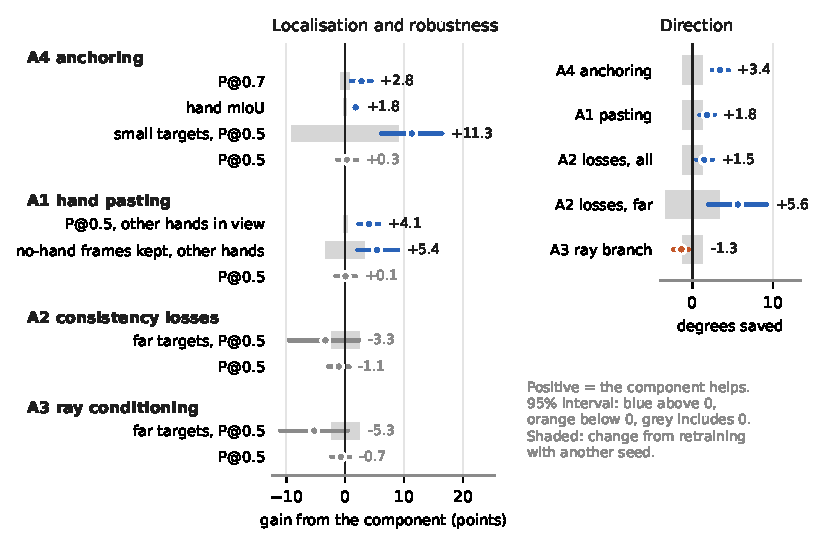
\includegraphics[width=\linewidth]{figures/ablation_effects}
  \caption{What each component contributes, with 95\% paired-bootstrap intervals. Gain = full model minus ablation, or degrees of direction error saved, so positive means the component helps. Grey bands: the largest change that retraining the full model with another seed produced on the same metric. For each component, the first rows show the capability it was designed for and the last row shows P@0.5. ``Far'' in the labels denotes large-gap targets. The P@0.7 effect of A4 is not significant on the duplicate-free test split (Table~\ref{tab:ablation}).}
  \Description{Interval plot with grey bands for retraining variation. Anchoring: P@0.7 +2.8, hand mIoU +1.8, small targets +11.3, all above zero and outside the bands; P@0.5 +0.3, crossing zero. Hand pasting: P@0.5 with other hands +4.1 and no-hand frames kept +5.4, above zero; P@0.5 +0.1. Consistency losses and ray conditioning: far-target and overall P@0.5 effects cross zero. Direction panel: degrees saved by anchoring 3.4, pasting 1.8, consistency losses 1.5 overall and 5.6 for far targets, all above zero; the ray branch -1.3, below zero.}
  \label{fig:ablation}
\end{figure}

\paragraph{No component changes coarse accuracy.} All four variants stay within ${\pm}1.1$ points of the full model's P@0.5 (58.9\%), and none differs significantly; retraining alone moves P@0.5 by 0.1 points, so we draw no conclusions from P@0.5 differences. The components differ instead in the capabilities they add, at a cost of at most 13K parameters each.

\paragraph{A4, instance anchoring: a more precise hand box and direction.} Against a plain model of the same size, the anchored chain improves hand mIoU by 1.8 points [+1.4, +2.2], against at most 0.3 between seeds, and lowers the direction error by 3.4$^\circ$ [2.4, 4.5], against at most 1.2$^\circ$. It also raises P@0.7 by 2.8 points [+1.1, +4.3] and small-target P@0.5 by 11.3 points [+6.5, +16.5] (the plain model's small boxes are drawn 2.4 instead of 1.9 times too large), but we treat these two as supporting evidence only: without duplicated test images the P@0.7 gain shrinks to 1.7 [0.0, +3.5], and the small-target gain is close to the seed spread (9.1). A plain model therefore finds the right region as often, but with a less precise hand box and direction. A4 also stopped earliest (best epoch 54, against 100), so its effects include a different training length.

\paragraph{A1, distractor pasting: robustness to synthetic other hands.} With other hands in view, the model trained with pasting keeps 4.1 more points of target P@0.5 [+2.4, +5.8] and 5.4 more points of no-hand frames as \emph{no hand} [+1.9, +8.9], and it puts its hand on another person's hand six times less often (0.2\% against 1.2\%). On clean images it costs nothing (P@0.5 $-$0.1) and even helps slightly (mIoU +1.2, hand mIoU +0.6, and 1.8$^\circ$ less direction error), which is consistent with pasting acting as a regulariser that makes the model rely on the hand's position and context rather than on its appearance alone. The ownership-accuracy metric itself barely moves (99.7\% against 98.7\%), because pasted hands sit higher in the frame than the wearer's (Section~\ref{sec:own}).

\paragraph{A2, consistency losses: a sharper direction, not a better box.} Without the two consistency terms, the direction error for large-gap targets rises by 5.6$^\circ$ [+2.1, +9.4], to 34.6$^\circ$, above all three seeds of the full model (29.0--32.3$^\circ$); this is where the ray-alignment term weighs most. Overall, the direction error rises by 1.5$^\circ$, only slightly more than retraining alone changes it (1.2$^\circ$). Target-box accuracy does not change ($+$1.1 P@0.5, n.s.), because the target head does not draw on the predicted direction (A3 below). The losses therefore sharpen an output that an interface can use directly, for example to draw the pointing ray as feedback, but not the box.

\paragraph{A3, explicit ray geometry: what a small model learns from it.} Removing the ray branch $G^t$ changes P@0.5 by less than one point ($+$0.7, n.s.). P@0.7 rises by 1.9 points [+0.2, +3.6] and the direction error falls by 1.3$^\circ$, both outside the seed spread, but the P@0.7 gain does not survive the duplicate check ($+$1.6 [$-$0.2, +3.3]), and A3 also trained 20\% longer (best epoch 120). Probing the trained full model suggests why the branch adds nothing. The model does rely on it: its output is as large as the visual term (median ratio of spreads 0.86 on 500--800 test images), and switching it off at inference lowers P@0.5 on the whole test split from 58.9\% to 50.6\%. But it has learned proximity more than direction: its output correlates more with closeness to the fingertip ($\rho=-0.38$) than with closeness to the ray's line ($-0.27$), and on the probe subset hardly at all with being in front of the fingertip ($+0.04$). Accordingly, switching it off costs 11 points of P@0.5 on overlap targets and 9.5 on near ones in the probe subset, while on large-gap targets of the whole test split P@0.5 even rises by 2.0 points. A plausible reason is the training distribution: with 70\% overlap and 7\% large-gap targets, a ``near the fingertip'' prior already fits most targets, and the visual head can learn it by itself. The branch can therefore be dropped without loss. We keep it in the deployed model because that is the model measured on the glasses. The next paragraph tests the two remedies this analysis suggests.

\paragraph{Testing the remedies.} We retrained the 160\,px model three more times, each with one change and the seed and settings of the main run (Table~\ref{tab:remedies}). E1 lets the learned ray prior act only in front of the fingertip ($G^t$ is set to zero wherever $t_k<0$). E2 weights the target-box and target-heatmap losses three times as much for near and large-gap targets, the 30\% of training images in which the fingertip does not overlap the target. E3 spaces the $3\times3$ sample that predicts the target size two cells apart, so that it covers 40 instead of 24 pixels; none of the three adds a parameter.
\begin{itemize}
\item \emph{Neither remedy for large-gap targets works.} Constraining the prior to point forward (E1) leaves P@0.5 unchanged; large-gap P@0.5 rises by 5.3 points, but the interval includes zero ([$-$0.5, +11.0]), and the direction error for large-gap targets grows by 4.3$^\circ$. Up-weighting non-overlap targets (E2) trades overlap accuracy for gains that are not significant: overlap P@0.5 falls by 3.8 points and overall P@0.5 by 1.8, while near and large-gap P@0.5 rise by 2.0 and 3.8 points with intervals that include zero; the hand box and the overall direction also become less precise (hand mIoU $-$1.2, direction error $+$2.5$^\circ$).
\item \emph{A wider size sample does not tighten the boxes.} With the size sample spaced two cells apart (E3), P@0.7 changes by $-$1.2 points and small-target P@0.5 by $+$1.3, both with intervals that include zero, while the hand box and the large-gap direction become slightly less precise. Box extent is therefore not limited by how far the size head looks around the predicted centre; a different size head, closer to the multi-scale box regression of detectors, is left to future work.
\end{itemize}
Together with A2, A3 and the flat direction error across resolutions, these results locate the remaining bottleneck for large-gap targets in how the direction is estimated, not in how the ray prior is shaped or how the training images are weighted. A direction supervised by the finger's own axis, for example from finger keypoints, remains untested.

\begin{table}[t]
  \caption{Remedies tested at 160\,px (one seed each; no extra parameters). Differences from the full model, in points (degrees for the direction error, where positive means worse); brackets: 95\% paired-bootstrap interval. Bold: the interval excludes 0 and the difference exceeds the largest change between the three seeds of the full model (P@0.5 0.1, P@0.7 0.8, overlap 0.5, large gap 2.4, small 9.1, hand mIoU 0.3, large-gap direction 3.4$^\circ$). Best epoch in parentheses (full model: 100).}
  \label{tab:remedies}
  \footnotesize
  \setlength{\tabcolsep}{2.5pt}
  \begin{tabular}{lrrrrrrr}
    \toprule
    Variant & P@0.5 & P@0.7 & Overlap & Large gap & Small & Hand mIoU & Dir.\ large gap ($^\circ$) \\
    \midrule
    Full model & 58.9 & 31.8 & 66.0 & 25.4 & 36.9 & 73.7 & 29.0 \\
    \midrule
    E1 forward-only ray prior (78) & $+$0.3 & $+$0.2 & $-$0.4 & $+$5.3 {\scriptsize[$-$0.5, +11.0]} & $-$4.2 & \textbf{$-$0.8} & \textbf{$+$4.3} \\
    E2 non-overlap targets $\times3$ (65) & \textbf{$-$1.8} & \textbf{$-$3.7} & \textbf{$-$3.8} & $+$3.8 {\scriptsize[$-$1.9, +9.6]} & $-$3.6 & \textbf{$-$1.2} & $-$0.8 \\
    E3 size sample spaced 2 cells (82) & $+$0.2 & $-$1.2 & $-$0.8 & $+$3.4 {\scriptsize[$-$2.4, +9.6]} & $+$1.3 & \textbf{$-$0.6} & \textbf{$+$3.7} \\
    \bottomrule
  \end{tabular}
\end{table}

\paragraph{Robustness of these conclusions.} Every difference reported above as an effect is significant under the paired bootstrap and larger than the change produced by retraining with another seed; effects close to that threshold (the small-target gain of anchoring, and the overall direction changes of A1--A3, 1.3--1.8$^\circ$ against 1.2$^\circ$) are supporting evidence only. Removing duplicated test images changes no conclusion except the P@0.7 effects of A3 and A4. The loss weights were not searched (Appendix~\ref{app:weights}); A2 covers the two non-standard terms, and the remaining eleven are standard box, keypoint, heatmap and focal losses. Finally, replacing the backbone with MobileNetV3-Small~\cite{howard2019mobilenetv3} or MobileNetV4-Conv-Small~\cite{qin2024mobilenetv4} does not change P@0.5 significantly while doubling or nearly tripling the parameters (Appendix~\ref{app:extra}), so ShuffleNetV2 0.5$\times$ is the efficient choice at this scale.

\subsection{Other People's Hands in View}\label{sec:own}

With one or two pasted hands in each test image (Table~\ref{tab:own}), the model's hand still lies nearer the wearer's hand than any pasted hand in 99.7\% of hand images, and target P@0.5 does not drop (60.1\% against 58.9\% on clean images). This ownership metric is easy under the synthetic distribution: pasted hands sit in the upper part of the frame and the wearer's hand in the lower part, so ownership accuracy on training batches was already 93\% in the first epoch, when the hand IoU was only 0.38. Two numbers are more informative. Pasted hands rarely turn a no-hand frame into a hand frame: 91.8\% of no-hand frames stay \emph{no hand}, against 93.4\% without pasted hands. And the training recipe is needed: without it (A1), target P@0.5 with other hands in view drops by 4.1 points and no-hand frames kept drop by 5.4, while clean accuracy is unchanged. The compact detectors of Section~\ref{sec:detectors}, trained without pasting, lose 2.4--4.6 points under the same pasted hands, but YOLO26n trained with our pasting is as stable as SpatialNet (Table~\ref{tab:controlled}): the robustness to synthetic other hands comes from the training recipe and transfers to a generic detector. EgoPoint contains no real frames with other people's hands, and we did not record any, so robustness to real bystander hands remains untested.
%% Optional, only if part G3 of the device request (companions' hands in view) comes back: add the ownership
%% accuracy on those frames here, with a Wilson interval and Cohen's kappa, and a row to Table tab:own.

\begin{table}[t]
  \caption{Ownership on test images with one or two pasted hands. All values in \%. \emph{On other hand}: predicted hand centre inside a pasted hand. \emph{No hand kept}: no-hand images still classed as no hand, at the hand-gate threshold of 0.5.}
  \label{tab:own}
  \footnotesize
  \begin{tabular}{lrrrr}
    \toprule
    & Ownership accuracy & On other hand & No hand kept & Target P@0.5 \\
    \midrule
    Full model, clean test images & -- & -- & 93.4 & 58.9 \\
    Full model, pasted hands & 99.7 [99.4, 99.9] & 0.2 & 91.8 & 60.1 \\
    A1 (no pasting), pasted hands & 98.7 [98.2, 99.1] & 1.2 & 86.4 & 56.1 \\
    \bottomrule
  \end{tabular}
\end{table}

\subsection{On-Device Performance}\label{sec:ondevice}

Table~\ref{tab:device} reports cost on the evaluation machine and on the glasses.

\begin{table}[t]
  \caption{Inference cost of the 160\,px model. Server rows: PyTorch eager mode, batch size 1, on the 4-core Kaggle virtual machine used for evaluation (reference only; at this model size they are dominated by framework overhead). Glasses rows: the engineering unit of Section~\ref{sec:device}; battery rows are single one-minute observations. $^\ast$\,Derived from the per-frame latency, assuming frames are processed back to back.}
  \label{tab:device}
  \footnotesize
  \begin{tabular}{lr}
    \toprule
    Platform and measure & Value \\
    \midrule
    Server CPU, 1 thread: latency, median / p90 & 25.7 / 28.0\,ms \\
    Server CPU, 4 threads: latency, median / p90 & 25.8 / 27.0\,ms \\
    Server GPU, NVIDIA Tesla T4: latency, median / p90 & 15.9 / 16.3\,ms \\
    \midrule
    Glasses: inference latency per frame & 60--80\,ms \\
    Glasses: throughput$^\ast$ & 12--17 frames/s \\
    Glasses: peak additional RAM during inference & ${\approx}$100\,KB \\
    Glasses: battery drain in one minute, SpatialNet running continuously & 9\% \\
    Glasses: battery drain in one minute, streaming frames to the phone at 0.5\,fps & 16\% \\
    \bottomrule
  \end{tabular}
\end{table}

\paragraph{Latency and memory.} SpatialNet takes 60--80\,ms per frame on the glasses, within the 100--200\,ms commonly targeted for interactive response~\cite{miller1968response,card1991information}, which allows 12--17 frames per second. Inference needs about 100\,KB of RAM beyond the idle application with the model loaded, and the FP16 weights take 1.6\,MB. Running the weights in half precision gives the same target IoU as FP32 on 320 validation images (0.510 in both), so halving the model size costs no accuracy.

\paragraph{Battery (one observation per mode).} Over one minute on the engineering unit, continuous inference used 9 percentage points of charge, and streaming frames to the phone at 0.5\,fps used 16, although the streaming mode sends only one frame every two seconds while SpatialNet processes frames continuously. Each mode was measured once, the fuel gauge resolves 1\%, and the unit has no production power management, so this indicates the relative cost of the two modes on this unit only. It is neither an energy measurement nor a battery-life estimate, and continuous inference is the worst case: in use, the model would run only while the wearer is pointing.

\paragraph{Scope of the device results.} The 224 and 320\,px models and the compact detectors were not measured on the glasses; the higher-resolution models need two and four times the compute of the deployed one. Section~\ref{sec:realframes} checks the deployed model's accuracy on frames from the glasses' camera.

\subsection{Frames from the Glasses' Camera}\label{sec:realframes}

All accuracy figures above come from EgoPoint. The deployed camera differs: its frames are portrait and squashed to a square (Section~\ref{sec:device}), and they come from other people, places and objects. As a check of transfer, \tbd{K} wearers recorded \tbd{N} frames with the glasses while pointing at everyday objects, at different distances, in \tbd{places}, and \tbd{M} frames with no hand in view. For each pointing frame, the wearer named the object they meant; afterwards, \tbd{two annotators} drew the box of that object and of the wearer's hand without seeing the model's outputs. We score the outputs that the model produced on the glasses with the metrics of Section~\ref{sec:metrics}, with Wilson intervals (Table~\ref{tab:real}); Figure~\ref{fig:real} shows examples. \tbd{One or two sentences on the result: whether hand P@0.5, target P@0.5 and centre in target stay close to the EgoPoint values, how many targets had a large gap, and which failure types of Section~\ref{sec:qual} appear.} With \tbd{N} frames, this check can reveal a large drop in accuracy but not a small one.

\begin{table}[t]
  \caption{The deployed model on EgoPoint and on frames from the glasses' camera, scored with the same metrics. Accuracy in \%; brackets: 95\% Wilson intervals. \emph{Centre in}: predicted target centre inside the annotated box. \emph{No hand kept}: frames without a hand classed as no hand, at the hand-gate threshold of 0.5.}
  \label{tab:real}
  \footnotesize
  \begin{tabular}{lrrrrr}
    \toprule
    Frames & Pointing / no hand & Hand P@0.5 & Target P@0.5 & Centre in & No hand kept \\
    \midrule
    EgoPoint test split & 2,604 / 425 & 92.6 & 58.9 & 84.8 & 93.4 \\
    Glasses' camera & \tbd{N} / \tbd{M} & \xx\ [\xx, \xx] & \xx\ [\xx, \xx] & \xx\ [\xx, \xx] & \xx\ [\xx, \xx] \\
    \bottomrule
  \end{tabular}
\end{table}

\begin{figure}[t]
  \centering
  \phfig{\linewidth}{3.2cm}{Six frames from the glasses' camera with SpatialNet's on-device outputs (hand, fingertip, ray, target) and the annotated target. Include at least one failure.}
  \caption{Frames from the glasses' camera. \tbd{Insert after the real-frame check.}}
  \Description{To be inserted: six photos from the glasses showing SpatialNet's outputs and the annotated target.}
  \label{fig:real}
\end{figure}

\subsection{Qualitative Results and Failure Analysis}\label{sec:qual}

We sorted the 558 test images with target IoU $<$ 0.3 (21.4\%) by rule. In 36\%, the model found the right object but drew the wrong extent: the predicted centre lies inside the labelled box, mostly for overlap targets (137 of 199), for example part of a bed instead of the whole bed. In 33\%, the direction was wrong (error over 45$^\circ$). In 31\%, the model chose the wrong object despite a reasonable direction, mostly for near and large-gap targets (130 of 171), typically a similar object next to the labelled one along the ray. In 1\%, the hand was missed. Appendix~\ref{app:extra} shows one example of each type. Some labels are ambiguous: in the ``wrong direction'' example, the finger touches a bowl while the label is an apple above it. Such cases count as failures in every metric, for our model and the compared models alike.

Figure~\ref{fig:failures} shows four deliberately selected complex scenes. Repeated tableware and a dense bookshelf create look-alike neighbours, and the model boxes an adjacent stack or book (a, b). In a cluttered garden, the box takes in surrounding plants instead of the small labelled object (c). In a harbour scene with several depth layers, the model boxes a foreground region instead of the labelled boat (d). In all four, the wearer's hand and fingertip are found; the failure lies in deciding which object is meant and how far it extends. These examples illustrate failure types, not how often they occur.

\begin{figure}[t]
  \centering
  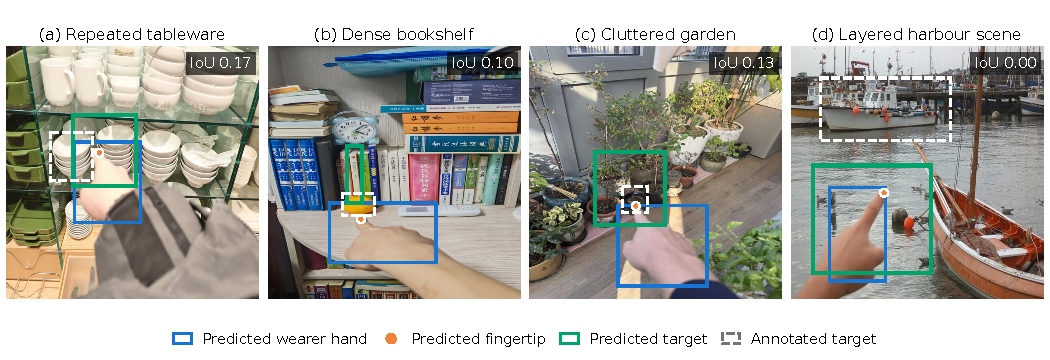
\includegraphics[width=\linewidth]{figures/failures_complex}
  \caption{Selected complex failures: repeated tableware (a) and a dense bookshelf (b) create look-alike neighbours; foliage complicates the target's extent (c); several depth layers separate the fingertip from the labelled boat (d). Colours as in Figure~\ref{fig:teaser}; boxes, points and IoUs are the saved test predictions of the 160\,px model.}
  \Description{Four egocentric photos where the predicted target box misses the labelled one: a box on the wrong stack of tableware in a glass cabinet (IoU 0.17), a box on a neighbouring book in a dense bookshelf (IoU 0.10), a box covering plants around a small object in a garden (IoU 0.13), and a foreground box instead of a distant boat in a harbour (IoU 0.00). The wearer's hand and fingertip are found in all four.}
  \label{fig:failures}
\end{figure}

\section{Discussion}\label{sec:discussion}

\paragraph{What a small model can and cannot do.} Finding the wearer's hand, the fingertip and whether a hand is present works at this size (hand P@0.5 of 92.6\%, 3.9\,px fingertip error, AUROC 0.998), although compact detectors draw the hand box more tightly. Deciding which object the finger refers to, and how far that object extends, is what large models do much better; compact detectors of the same compute pick the object slightly less often than SpatialNet but draw its extent much better, even with the same ImageNet pretraining (Section~\ref{sec:detectors}). EgoPoint is dominated by overlap: in about 70\% of images the fingertip lies inside the target box, so for most targets the fingertip tells \emph{where} the object is but not \emph{how large} it is (a mean-size box at the true fingertip reaches 11.4\% P@0.5). One possible reason is that people align the fingertip with the target from the eye~\cite{mayer2015modeling,plaumann2018towards}, so that a camera next to the eye sees the target at or just behind the fingertip; because 61\% of EgoPoint images are composed or generated (Section~\ref{sec:data}), this remains a hypothesis about real pointing. Large-gap targets, where the ray matters, are only 7\% of the data. That is too few to shape a learned ray prior, and it is where errors concentrate.

\paragraph{Design implications.} For pointing interfaces on glasses, our results suggest six practical rules.
\begin{enumerate}
\item \emph{Choose the model by what the interface needs.} For a tight target box, a compact detector trained on pointing data is more accurate at the same compute, even without COCO pretraining. For naming the target, a structured model did as well, and it also provides the hand, the fingertip and the direction for feedback or gating in the same pass (Section~\ref{sec:detectors}).
\item \emph{Train with distractor hands, whatever the model.} Pasting unlabelled hands into the training images makes SpatialNet and a generic detector equally stable when other hands are in view, at no cost on clean images (Section~\ref{sec:detectors}).
\item \emph{Spend extra compute on resolution first.} At similar extra compute, a larger input gained more than a larger backbone (Sections~\ref{sec:resolution} and~\ref{sec:ablations}).
\item \emph{Confirm large-gap selections}, for example by naming or highlighting the target before acting on it, because errors concentrate there; for these targets, a recogniser does about as well with the whole frame as with SpatialNet's crop (Sections~\ref{sec:detectors} and~\ref{sec:heads-results}).
\item \emph{Smooth over time before triggering.} Per-frame false alarms make single-frame triggering unreliable (Section~\ref{sec:heads-results}).
\item \emph{Keep frames on the device.} A later recogniser needs only the target crop (Section~\ref{sec:problem}), which limits computation, bandwidth and the bystander imagery that leaves the glasses. On our unit, continuous local inference also used less charge than streaming frames to the phone, although one-minute observations do not establish an energy advantage (Section~\ref{sec:ondevice}).
\end{enumerate}

\paragraph{Limitations.}
\begin{itemize}
\item \emph{Construct validity.} The gap categories are image-plane relations. The direction label runs from the fingertip to the target centre, not along the finger, so direction errors mix pointing geometry with the choice of target centre. The ray lives in the image plane, so objects at different depths along the same image ray are told apart only by appearance, and the eye--camera offset is ignored.
\item \emph{Internal validity.} The ablation, resolution and backbone variants are single runs whose checkpoints come from different epochs (54 to 120), and some interventions are bundled (A1, A2 and A4). Paired intervals capture test-sample variation, not training randomness, and the per-component reading of the ablations is exploratory. Early stopping ended the one-cycle schedule before it completed.
\item \emph{External validity.} All accuracy figures come from one dataset with mostly landscape, partly composed or generated images, 4.7\% of whose test images duplicate training or validation images, and with unknown demographic coverage (for example, skin tone and handedness; flipping covers left hands only geometrically). Frames are squashed to a square, and the glasses' camera is portrait. EgoPoint has no non-pointing hands and no pointing without a target, so the pointing and target gates are untested, and in deployment a non-pointing hand may be read as pointing. The model has no temporal context. Our distractors are synthetic and encode the prior that the wearer's arm enters from the bottom of the view; a raised arm, or a companion's hand near the bottom, can break it, and we did not test real frames with other people's hands. The check on frames from the glasses (Section~\ref{sec:realframes}) covers only the wearer's hand and is small.
\item \emph{Baselines and measurement.} We copied the published large-model results and did not re-run any multimodal LLM under our protocol; the compact detectors we did train draw better boxes at the same compute. COCO-pretrained detectors have seen the source photographs of at least 41\% of our test images, but COCO pretraining gave YOLO26n no extra gain on them; published models trained on large image collections may have seen them too, which we could not test. The remedies, the ablations and three of the four controlled detector runs used one training seed each. The recognition test is category-level, uses two zero-shot recognisers, and measures what a recogniser receives, not what a user experiences. Within EgoPoint itself, 230 test images share their source photograph with a training or validation image. The device measurements are single observations on a pre-production unit, and we did not measure the detectors on the glasses. Finally, we measure the model on a benchmark and on the device, not the interaction: how wearers respond to its errors, and which confirmation designs suit them, need a study with participants wearing the glasses.
\end{itemize}

\section{Ethics and Privacy}\label{sec:ethics}

\paragraph{Bystanders.} A head-worn camera sees people who did not consent to being recorded, and bystanders' concerns about camera glasses are well documented~\cite{denning2014situ,hoyle2014privacy}. SpatialNet runs on the glasses, so localisation needs no frame to leave the device, and a downstream step can be limited to the target crop and to moments when the wearer points. SpatialNet is trained to ignore other people's hands; it does not detect, identify or track people. On-device processing still does not remove the need for visible recording indicators; the test unit has user- and bystander-facing LEDs.

\paragraph{Data.} EgoPoint is used under the access terms of its authors' release, for research only. We do not redistribute its images or our converted labels; our conversion script regenerates the labels from the original release. The images shown in this paper come from its test and training splits. \tbd{Real-frame check (Section~\ref{sec:realframes}): state who recorded the frames and how they consented, the ethics approval or exemption, how long the frames are kept, and how bystanders were kept out of view or blurred.}

\paragraph{Availability.} We will release the code, the dataset conversion script, the trained weights and the per-image evaluation outputs, from which every table can be recomputed, upon publication.

\section{Conclusion}\label{sec:conclusion}
SpatialNet localises the object a smart-glasses wearer points at from one RGB frame, with one forward pass of a 0.72M-parameter CNN and no prompt, language model or external pose model, and it runs on a pre-production pair of glasses in 60--80\,ms per frame. It finds the wearer's hand and fingertip reliably and the pointed-at object with a P@0.5 of 58.9\%, but only 25.4\% for large-gap targets. That is well below large GPU models, and compact detectors of the same compute, even with the same ImageNet pretraining, draw tighter boxes, although SpatialNet places its target on the labelled object more often, and an off-the-shelf recogniser names the target from its crops as often as from theirs, except when the target lies far from the fingertip. SpatialNet is also smaller and returns the hand, fingertip and direction from the same pass. Its pasted-hand training keeps it stable when synthetic hands are in view, and does the same for a generic detector. Its instance-anchored heads make the hand box and the direction more precise than a plain model of the same size, and input resolution is the largest further lever. An explicit ray prior learns mainly fingertip proximity when most targets overlap the fingertip, and neither a forward constraint nor re-weighting large-gap targets corrects it. Finally, at least 41\% of the EgoPoint test images are COCO photographs; COCO pretraining did not exploit this in our runs, but benchmarks on this dataset should report it. The main open problems are pointing scenes that EgoPoint does not contain, real bystander hands, and large-gap targets along ambiguous rays. We expect progress on them to come from richer egocentric pointing data at least as much as from larger models.


\bibliographystyle{ACM-Reference-Format}
\bibliography{references,references-revision}

\appendix
\section{Loss Weights}\label{app:weights}

Table~\ref{tab:weights} lists the 13 loss terms and their weights. The weights were set by hand during development, using the training and validation splits only, and were not tuned by a search. Ablation A2 (Section~\ref{sec:ablations}) removes the two non-standard terms; the others are standard box, keypoint, heatmap and focal losses.

\begin{table}[h]
  \caption{Loss terms, their supervision, and weights.}
  \label{tab:weights}
  \footnotesize
  \begin{tabular}{llll}
    \toprule
    Term & Loss & Supervision & Weight \\
    \midrule
    Hand box & 1 $-$ CIoU & hand box & 0.10 \\
    Fingertip & Wing ($w{=}0.5$, $\epsilon{=}0.1$) & fingertip & 0.18 \\
    Direction & 1 $-$ cosine & fingertip $\to$ target centre & 0.03 \\
    Target box & 1 $-$ SIoU & target box & 0.45 \\
    Target box, auxiliary & 1 $-$ IoU & target box & 0.10 \\
    Hand gate & focal BCE, positives $\times3$ & $H$ & 0.08 \\
    Pointing gate & focal BCE, positives $\times2$ & $P$ (hand images) & 0.10 \\
    Target gate & focal BCE, positives $\times2$ & $T$ (pointing images) & 0.06 \\
    Ray alignment & distance to ray $+$ 0.5 $\cdot$ behind & none (predictions only) & 0.08 \\
    Hand axis & hinge outside a $60^\circ$ cone & none (predictions only) & 0.02 \\
    Hand heatmap & penalty-reduced focal, ownership-weighted & hand centre & 0.10 \\
    Fingertip heatmap & penalty-reduced focal & fingertip & 0.10 \\
    Target heatmap & penalty-reduced focal & target centre & 0.10 \\
    \bottomrule
  \end{tabular}
\end{table}

\section{Augmentation Parameters}\label{app:aug}

\begin{table}[h]
  \caption{Training-time augmentation, applied on the fly; each training image is seen once per epoch as a new random variant. Validation and test images are only resized and normalised.}
  \label{tab:aug}
  \footnotesize
  \begin{tabular}{lp{0.62\linewidth}}
    \toprule
    Step & Setting \\
    \midrule
    Distractor hands & 1--2 hands with probability 0.5 (hand images) or 0.3 (no-hand images); scale 0.45--1.0; rotation by 90/180/270$^\circ$ and optional mirror with probability 0.7; centre in the top 65\% of the frame; overlap with the wearer's hand and the target below 15\%; feathered alpha (12\% of the crop size); colour jitter; 30\% self-paste; pool of 512 donor crops, half from pointing hands \\
    Decoy patch & unlabelled non-hand patch from a no-hand image, with probability 0.15 \\
    Horizontal flip & 0.5 \\
    Shift / scale / rotate & ${\pm}5\%$ / ${\pm}10\%$ / ${\pm}15^\circ$, probability 0.4 \\
    Perspective & scale 0.02--0.05, probability 0.2 \\
    Brightness / contrast & ${\pm}20\%$, probability 0.5 \\
    Gaussian blur & kernel 3--5, probability 0.2 \\
    Mixup & within the same scene, $\lambda\sim\mathrm{Beta}(0.2,0.2)$ folded to ${\geq}0.5$, label of the dominant image, every batch \\
    Anchor forcing & ground-truth anchors with probability 0.5 decaying to 0 over 20 epochs \\
    \bottomrule
  \end{tabular}
\end{table}

\section{Additional Results}\label{app:extra}

\paragraph{Backbone.} Table~\ref{tab:backbone} replaces the ShuffleNetV2 0.5$\times$ backbone with MobileNetV3-Small~\cite{howard2019mobilenetv3} or MobileNetV4-Conv-Small~\cite{qin2024mobilenetv4}, with the recipe otherwise unchanged. Neither changes P@0.5 significantly, while doubling or nearly tripling the parameters. Both lean towards better large-gap accuracy (+5.7 and +4.8 points, intervals across 0) and a lower fingertip error (3.5 against 3.9\,px). Both runs stopped earlier (best epoch 64, against 100), so their numbers may be slightly low.

\begin{table}[h]
  \caption{Backbone swap at 160\,px, main-run recipe otherwise unchanged (one seed each). Target metrics in \%; brackets: 95\% paired-bootstrap interval of the difference from ShuffleNetV2.}
  \label{tab:backbone}
  \footnotesize
  \setlength{\tabcolsep}{4pt}
  \begin{tabular}{lrrrrrr}
    \toprule
    Backbone & Params & FP16 & GFLOPs & P@0.5 & Large-gap P@0.5 & Fingertip \\
    \midrule
    ShuffleNetV2 0.5$\times$ (ours) & 0.72M & 1.6\,MB & 0.231 & 58.9 & 25.4 & 3.9\,px \\
    MobileNetV3-Small & 1.57M & 3.2\,MB & 0.255 & 58.1 [$-$2.7, +1.0] & 31.1 [$-$0.5, +12.0] & 3.5\,px \\
    MobileNetV4-Conv-Small & 1.99M & 4.1\,MB & 0.398 & 59.8 [$-$0.9, +2.8] & 30.1 [$-$1.0, +10.5] & 3.5\,px \\
    \bottomrule
  \end{tabular}
\end{table}

\paragraph{IoU success curves.} Figure~\ref{fig:curves} shows how the share of successful hand and target boxes falls with the IoU threshold.

\begin{figure}[h]
  \centering
  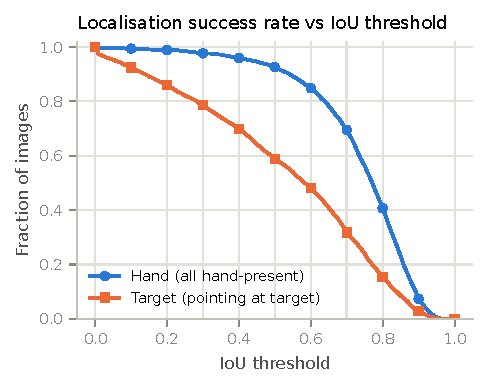
\includegraphics[width=0.48\linewidth]{figures/results/iou_success_rate}
  \caption{Share of test images whose hand or target box reaches each IoU threshold.}
  \Description{Two curves of success rate against IoU threshold; the hand curve stays above 0.9 up to IoU 0.5 and falls after 0.7, while the target curve falls steadily, reaching 0.59 at IoU 0.5 and 0.32 at 0.7.}
  \label{fig:curves}
\end{figure}

\paragraph{Failure types.} Figure~\ref{fig:qual} shows typical successes and one example of each failure type of Section~\ref{sec:qual}.

\begin{figure}[h]
  \centering
  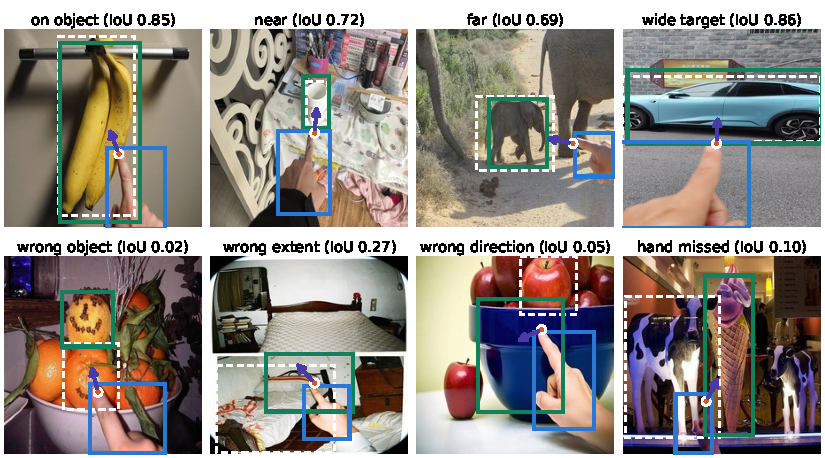
\includegraphics[width=\linewidth]{figures/qualitative}
  \caption{Successes (top) and failures (bottom) on EgoPoint test images: predicted hand (blue), fingertip and direction, and target (green); labelled target dashed. Bottom row, one example per failure type of Section~\ref{sec:qual}.}
  \Description{Eight egocentric images. Top row: correct target boxes for bananas touched by the finger, a cup near the finger, a young elephant far from the finger, and a car. Bottom row: a box on the wrong orange in a bowl of oranges, a box on part of a bed instead of the labelled bed, a box on a bowl while the label is an apple above it, and a frame where the hand gate missed the hand.}
  \label{fig:qual}
\end{figure}


\end{document}
